\PassOptionsToPackage{table}{xcolor}
\documentclass[12pt]{article}

\usepackage{sbc-template}
\usepackage{graphicx,url}
\usepackage[utf8]{inputenc}
\usepackage[english]{babel}
\usepackage{booktabs}
\usepackage{array}
\usepackage{amsmath}
\usepackage{tikz}
\usetikzlibrary{arrows.meta,positioning,fit,backgrounds,calc}
\usepackage{pgfplots}
\pgfplotsset{compat=1.16}
\definecolor{accent}{HTML}{2a78d6}
\definecolor{context}{HTML}{52514e}
\definecolor{ink}{HTML}{0b0b0b}
\definecolor{muted}{HTML}{8a8984}
\definecolor{accentfill}{HTML}{eaf2fc}
\definecolor{contextfill}{HTML}{f2f1ee}
\definecolor{gridline}{HTML}{d9d8d4}
%% cores semanticas das tabelas: queda e recuperacao
\definecolor{queda}{HTML}{fbe3e0}
\definecolor{alta}{HTML}{e2f0e4}
\definecolor{realce}{HTML}{eef1fb}
\definecolor{cabec}{HTML}{e8e7e3}


%% Ajuste de espaco para o formato short (6 pag.): um passo de fonte abaixo no
%% bloco autoral e nas referencias. Margens, corpo e tabelas ficam intactos.
\makeatletter
\def\@maketitle{\newpage
 \begin{center}
  \vspace*{-.7cm}
  {\XVIPT\bf\@title\par}
   \vglue 5pt plus 3pt minus 3pt
  {\small\textbf{\begin{tabular}[t]{c}\@author\end{tabular}}\par}
   \vglue 4pt plus 3pt minus 3pt
  {\small\begin{tabular}[t]{c}\inst{\instnum}\@address\end{tabular}\par}
   \vglue 5pt plus 3pt minus 3pt
 \end{center}\par
}
\makeatother

%% Aperto leve de espacamento para o formato short. Fontes do corpo, margens e
%% tabelas ficam intactas; so o espaco entre paragrafos e entre referencias cede.
\setlength{\parskip}{5pt}
\makeatletter
\let\@oldbibliography\thebibliography
\renewcommand{\thebibliography}[1]{\@oldbibliography{#1}%
  \setlength{\itemsep}{0pt}\setlength{\parsep}{0pt}\setlength{\parskip}{0pt}}
\makeatother

\sloppy

\title{SPIN-Seq: predicting the typed residue interaction\\
network from sequence}




\author{Wyllgner F. Amorim\inst{1}, Jáder L. S. Gonçalves\inst{2},\\
  Nicolas F. C. Sales\inst{3}, Andrey R. S. Riça\inst{3},
  Hemily U. dos Santos\inst{3},\\
  Thiago A. Guarnieri\inst{3}, Lucas M. da Cunha\inst{3}}



%% TODO: acrescentar ORCID e \email{} dos sete autores --- o BSB encoraja ORCID
%% (CFP 2024) e o \address do template SBC normalmente traz e-mail de contato.
\address{Professional and Technological Education Sector\\
  Federal University of Paraná (UFPR) -- Curitiba, PR -- Brazil
\nextinstitute
  Institute of Mathematical and Computer Sciences\\
  University of São Paulo (USP) -- São Carlos, SP -- Brazil
\nextinstitute
  Faculty of Engineering, Technology and Innovation\\
  Federal University of Rondônia (UNIR) -- Porto Velho, RO -- Brazil}

\begin{document}

\maketitle

\begin{abstract}
  Knowing which residues are close does not reveal how they interact. Residue interaction
  networks (RINs) label edges by chemistry, but established generators read 3D structures.
  SPIN-Seq predicts the typed intra-chain RIN over eight interaction types from sequence
  alone, with Arpeggio labels used only as targets. Over 5{,}176{,}314 test pairs of a
  cluster-disjoint split, a frozen ESM-2 encoder and a 939k-parameter head reach macro
  AUPRC 0.520, against 0.110 for amino-acid propensity. A \emph{perfect} contact map
  reaches only 0.132 and cannot rank types among contacts: its per-class AUPRC is
  prevalence over contact density, a constant 25-fold lift. The recipe was selected on
  this same evaluation, and the encoder was pretrained on a corpus likely containing the
  test sequences.
\end{abstract}


\section{Introduction}
\label{sec:intro}

Recent structure predictors~\cite{jumper2021alphafold,lin2023esm2} have greatly improved
geometric modelling, but residue proximity does not specify interaction chemistry. Residue interaction networks (RINs) encode this chemistry,
distinguishing salt bridges, aromatic stacking interactions and van der Waals contacts.
Typed edges improve downstream models~\cite{rithetge2026}, yet established typed-RIN
generators require 3D coordinates.

The immediate alternative is to fold the sequence and then profile the predicted
structure, which may propagate errors where chemical typing is most sensitive. Many types
depend on side-chain geometry, where dihedral error compounds outward from the backbone,
from ${\approx}14\%$ at $\chi_1$ to ${\approx}48\%$ at $\chi_3$ and largest for polar
residues~\cite{biophysj2025sidechains}: a backbone root-mean-square deviation near
1\,\AA{} does not guarantee a correct salt bridge. The central question is therefore how
much interaction chemistry is recoverable from the sequence itself, under the constraint
that every model input be sequence-derived and Arpeggio-derived labels serve only as
targets.

Several related lines of research address parts of this problem, but not the full setting. Generators such as
Arpeggio~\cite{jubb2017arpeggio} and RING~\cite{delconte2024ring} annotate typed
interactions but read coordinates. Contact prediction returns geometry, not chemical
type; the attention-derived map~\cite{rao2021attention} is used here as an input
channel, not as a competing method. Sequence-only methods predict \emph{individual} types, including
disulfide connectivity~\cite{ceroni2006disulfind} and hydrogen
bonds~\cite{zhou2022mapshb}, but each resolves one class over a pair subset already
restricted by a chemical rule. Sequence-based typing was shown for protein--ligand
pairs~\cite{pham2025linker}, a setting that requires the ligand as input, and annotating
a predicted structure is not direct prediction either. To the best of our knowledge, no \emph{learned}
method addresses the joint, multi-label prediction of intra-chain RIN types over the
full graph, from one sequence, without alignment, templates or an intermediate
structure.

The contributions are: \textbf{(i)} a formulation of sequence-only RIN prediction as
multi-label classification over eight types, evaluated on all pairs under a
cluster-disjoint split; \textbf{(ii)} evidence
that the RIN reduces to neither composition nor a contact map, not even a perfect one;
\textbf{(iii)} ablations and a learning curve that trace performance gains and point to
data volume as the likeliest bottleneck.

\begin{figure}[tb]
  \centering
  \resizebox{0.87\linewidth}{!}{%
\begin{tikzpicture}[
  x=1cm, y=1cm,
  font=\fontsize{6.4}{7.6}\selectfont, color=ink,
  capt/.style={font=\fontsize{6.2}{7.2}\selectfont, color=context, align=center},
  tag/.style={font=\fontsize{5.6}{6.6}\selectfont, color=muted, align=center},
  flow/.style={-{Straight Barb[length=2.4pt,width=3pt]}, draw=accent, line width=0.7pt},
  bus/.style={draw=accent, line width=0.7pt},
  sflow/.style={-{Straight Barb[length=2.4pt,width=3pt]}, draw=context, line width=0.7pt},
  sbus/.style={draw=context, line width=0.7pt},
  lead/.style={draw=muted, line width=0.35pt, dash pattern=on 1.4pt off 1.2pt},
]

% ============================================================ helpers
\newcommand{\lmap}[4]{%
  \foreach \rw in {0,...,#2}{\foreach \cl in {0,...,#2}{
    \draw[draw=gridline, line width=0.2pt]
      (\cl*#1, -\rw*#1) rectangle ({(\cl+1)*#1}, {-(\rw+1)*#1});}}
  \edef\fillist{#4}%
  \foreach \rw/\cl in \fillist{
    \fill[#3] (\cl*#1, -\rw*#1) rectangle ({(\cl+1)*#1}, {-(\rw+1)*#1});}
  \draw[draw=context, line width=0.55pt]
    (0,0) rectangle ({(#2+1)*#1}, {-(#2+1)*#1});
}
\def\ctc{0/3,3/0,1/5,5/1,2/2,4/4,5/5,1/1,3/4,4/3,0/6,6/0,6/6,2/5,5/2}
\def\hs{0.115}      % cell side of the head/target maps
\def\hw{0.805}      % map side (7 cells)
\def\bus{11.05}     % bus x: spine shared by both registers
\def\yc{2.25}       % y of the contact channel
\def\yt{0.75}       % y of the type channel (main)
\def\yd{-0.85}      % y of the distance channel

% ============================================================ REGISTRO SUPERIOR
\node[anchor=west, color=accent, font=\fontsize{6.6}{8}\selectfont]
  at (-0.15, 2.62) {INPUTS: sequence only};

% ---------- 1. sequencia ----------
\node[anchor=north west, inner sep=0] at (-0.15, 1.74)
  {\resizebox{2.5cm}{!}{%
%% Icon 1: sequence of test chain 6AVD_A (40 residues, 8 cysteines).
%% Highlighted cysteines are the nodes of the 4 disulfide bridges.
\begin{tikzpicture}[x=1pt,y=1pt]
\node[anchor=west,inner sep=0pt,font=\ttfamily\fontsize{6.4}{7.6}\selectfont]
  at (0,9) {G\,S\,A\,E\,I\,I\,R\,\textcolor{accent}{\textbf{C}}\,S\,G\,T\,R\,E\,\textcolor{accent}{\textbf{C}}\,Y\,A\,P\,\textcolor{accent}{\textbf{C}}\,Q\,K\,};
\node[anchor=west,inner sep=0pt,font=\ttfamily\fontsize{6.4}{7.6}\selectfont]
  at (0,0) {L\,T\,G\,\textcolor{accent}{\textbf{C}}\,L\,N\,A\,K\,\textcolor{accent}{\textbf{C}}\,M\,N\,K\,A\,\textcolor{accent}{\textbf{C}}\,K\,\textcolor{accent}{\textbf{C}}\,Y\,G\,\textcolor{accent}{\textbf{C}}\,V\,};
\end{tikzpicture}%%
}};
\node[capt, anchor=north] at (1.10, 0.46) {sequence\\\tiny 6AVD, test};

\draw[flow] (2.48, \yt) -- (2.98, \yt);

% ---------- 2. ESM-2 (trapezio = codificador) ----------
\begin{scope}[shift={(3.05, 0.75)}]
  \fill[accentfill, draw=accent, line width=0.8pt]
    (0,0.72) -- (1.55,0.42) -- (1.55,-0.42) -- (0,-0.72) -- cycle;
  \node[color=ink, align=center] at (0.78, 0.10) {ESM-2\\650M};
  \begin{scope}[shift={(0.78,-0.42)}, scale=0.85]
    \draw[draw=accent, line width=0.6pt] (-0.075,0.055) arc (180:0:0.075);
    \fill[accent] (-0.13,-0.10) rectangle (0.13,0.06);
  \end{scope}
  \node[tag, anchor=north] at (0.78, -0.62) {frozen\\1280-d};
\end{scope}

\draw[flow] (4.68, \yt) -- (5.62, \yt);

% ---------- 3. tensor de par ----------
\begin{scope}[shift={(5.95, 1.36)}]
  \def\cs{0.175}
  \foreach \k in {0,...,6}{\fill[accentfill, draw=accent, line width=0.3pt]
    (\k*\cs, 0.10) rectangle ({(\k+1)*\cs}, 0.26);}
  \node[tag, anchor=south, color=accent] at (0.61, 0.26) {$h_j$};
  \foreach \k in {0,...,6}{\fill[accentfill, draw=accent, line width=0.3pt]
    (-0.26, -\k*\cs) rectangle (-0.10, {-(\k+1)*\cs});}
  \node[tag, anchor=east, color=accent] at (-0.28, -1.05) {$h_i$};
  \lmap{\cs}{6}{white}{\ctc}
  \fill[accent] (4*\cs, -2*\cs) rectangle (5*\cs, -3*\cs);
  \node[capt, anchor=north, align=center] at (0.45, -1.32)
    {$L\times L$ map\\\tiny training: crops $64{\times}64$};
  % pilha de channels
  \begin{scope}[shift={(1.45, 0.10)}]
    \fill[accentfill, draw=accent, line width=0.5pt] (0,0) rectangle (1.35,-0.72);
    \node at (0.675,-0.36) {\tiny $h_i,\,h_j$};
    \node[tag, anchor=west, color=context] at (1.39,-0.36) {96};
    \fill[accentfill, draw=accent, line width=0.9pt] (0,-0.78) rectangle (1.35,-1.06);
    \node at (0.675,-0.92) {\fontsize{4.6}{5.2}\selectfont AA, no projection};
    \node[tag, anchor=west, color=context] at (1.39,-0.92) {24};
    \fill[contextfill, draw=context, line width=0.45pt] (0,-1.12) rectangle (1.35,-1.36);
    \node at (0.675,-1.24) {\tiny sep.};
    \node[tag, anchor=west, color=context] at (1.39,-1.24) {1};
    \fill[contextfill, draw=context, line width=0.45pt] (0,-1.42) rectangle (1.35,-1.66);
    \node at (0.675,-1.54) {\tiny contact};
    \node[tag, anchor=west, color=context] at (1.39,-1.54) {1};
    \node[capt, anchor=north] at (0.675,-1.74) {\textbf{122} channels};
  \end{scope}
  \draw[lead] (5*\cs,-2*\cs) -- (1.45,0.10);
  \draw[lead] (5*\cs,-3*\cs) -- (1.45,-1.66);
\end{scope}

\draw[flow] (8.95, \yt) -- (9.34, \yt);

% ---------- 4. ResNet 2D (pilha de tensores) ----------
\begin{scope}[shift={(9.40, 1.28)}]
  \foreach \kk/\oo in {3/0.30, 2/0.20, 1/0.10, 0/0.00}{
    \fill[accentfill, draw=accent, line width=0.5pt]
      ({\oo},{-\oo}) rectangle ({\oo+1.05},{-\oo-1.05});}
  \node[capt, anchor=north, align=center] at (0.52, -1.42)
    {ResNet 2D\\\tiny 12 blocks, 64 channels};
\end{scope}

% ---------- 5. barramento -> tres cabecas ----------
\draw[flow] (10.80, \yt) -- ({\bus-0.02}, \yt);
\draw[lead] (10.88, 0.80) -- (10.88, 1.32);
\node[tag, anchor=south east, color=context, align=right] at (10.99, 1.30)
  {$\tfrac12(x{+}x^{\!\top})$\\inference only};
\draw[bus]  (\bus, \yc) -- (\bus, \yd);
\foreach \yy in {\yc, \yt, \yd}{\draw[flow] (\bus, \yy) -- (11.31, \yy);}

\begin{scope}[shift={(11.35, {\yc+\hw/2})}]
  \lmap{\hs}{6}{contextfill}{\ctc}
  \node[capt, anchor=north] at ({\hw/2}, {-\hw-0.06}) {contact};
\end{scope}
\begin{scope}[shift={(11.35, {\yt+\hw/2})}]
  \foreach \kk/\oo in {7/0.28, 6/0.24, 5/0.20, 4/0.16, 3/0.12, 2/0.08, 1/0.04}{
    \fill[accentfill, draw=accent, line width=0.4pt]
      ({\oo},{-\oo}) rectangle ({\oo+\hw},{-\oo-\hw});}
  \begin{scope}\lmap{\hs}{6}{accent}{\ctc}\end{scope}
  \node[capt, anchor=north, color=accent] at ({\hw/2+0.14}, {-\hw-0.34})
    {\textbf{8 types}};
\end{scope}
\begin{scope}[shift={(11.35, {\yd+\hw/2})}]
  \lmap{\hs}{6}{contextfill}{\ctc}
  \node[capt, anchor=north] at ({\hw/2}, {-\hw-0.06}) {distance};
\end{scope}
\node[tag, anchor=south, color=context] at (9.92, 2.24)
  {\textbf{939,026} param.};

% ---------- 6. predicted typed RIN ----------
\draw[flow] (12.50, \yt) -- (12.88, \yt);
\node[anchor=north west, inner sep=0] at (12.96, 1.89)
  {\resizebox{3.7cm}{!}{%
%% Icon 3: typed RIN PREDICTED by the champion model (p>0.5) for 6AVD_A.
%% Geometry converted from the original vector: 98 real edges and 58 nodes;
%% the 4 thick covalent edges are the disulfide bridges.
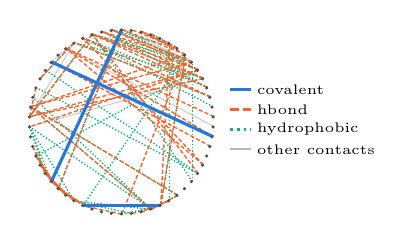
\begin{tikzpicture}[x=1pt,y=1pt]
\definecolor{rin0}{rgb}{0.5412,0.5372,0.5176}
\definecolor{rin1}{rgb}{0.1059,0.6863,0.4784}
\definecolor{rin2}{rgb}{0.9216,0.4078,0.2039}
\definecolor{rin3}{rgb}{0.1647,0.4706,0.8392}
\definecolor{rin4}{rgb}{0.3216,0.3176,0.3059}
\draw[rin0,line width=0.35pt,opacity=0.45] (9.342,23.213) -- (15.883,14.605);
\draw[rin0,line width=0.35pt,opacity=0.45] (68.384,54.511) -- (5.5,37.053);
\draw[rin0,line width=0.35pt,opacity=0.45] (64.326,60.495) -- (38.861,72.276);
\draw[rin0,line width=0.35pt,opacity=0.45] (72.226,37.053) -- (18.641,65.46);
\draw[rin0,line width=0.35pt,opacity=0.45] (21.634,67.491) -- (5.5,40.671);
\draw[rin0,line width=0.35pt,opacity=0.45] (21.634,67.491) -- (13.396,60.495);
\draw[rin1,line width=0.50pt,dash pattern=on 0.50pt off 0.70pt] (59.081,65.46) -- (35.251,72.08);
\draw[rin1,line width=0.50pt,dash pattern=on 0.50pt off 0.70pt] (64.326,17.23) -- (64.326,60.495);
\draw[rin1,line width=0.50pt,dash pattern=on 0.50pt off 0.70pt] (59.081,65.46) -- (49.531,70.524);
\draw[rin1,line width=0.50pt,dash pattern=on 0.50pt off 0.70pt] (64.326,60.495) -- (35.251,72.08);
\draw[rin1,line width=0.50pt,dash pattern=on 0.50pt off 0.70pt] (69.9,51.231) -- (24.832,69.185);
\draw[rin1,line width=0.50pt,dash pattern=on 0.50pt off 0.70pt] (69.9,51.231) -- (31.68,71.495);
\draw[rin1,line width=0.50pt,dash pattern=on 0.50pt off 0.70pt] (68.384,54.511) -- (28.195,70.524);
\draw[rin1,line width=0.50pt,dash pattern=on 0.50pt off 0.70pt] (71.833,44.266) -- (24.832,69.185);
\draw[rin1,line width=0.50pt,dash pattern=on 0.50pt off 0.70pt] (71.055,47.802) -- (21.634,67.491);
\draw[rin1,line width=0.50pt,dash pattern=on 0.50pt off 0.70pt] (64.326,60.495) -- (28.195,70.524);
\draw[rin1,line width=0.50pt,dash pattern=on 0.50pt off 0.70pt] (64.326,17.23) -- (28.195,70.524);
\draw[rin1,line width=0.50pt,dash pattern=on 0.50pt off 0.70pt] (38.861,72.276) -- (15.883,14.605);
\draw[rin1,line width=0.50pt,dash pattern=on 0.50pt off 0.70pt] (38.861,72.276) -- (13.396,17.23);
\draw[rin1,line width=0.50pt,dash pattern=on 0.50pt off 0.70pt] (66.518,57.611) -- (7.822,26.493);
\draw[rin1,line width=0.50pt,dash pattern=on 0.50pt off 0.70pt] (5.5,37.053) -- (11.208,20.113);
\draw[rin1,line width=0.50pt,dash pattern=on 0.50pt off 0.70pt] (66.518,57.611) -- (38.861,72.276);
\draw[rin1,line width=0.50pt,dash pattern=on 0.50pt off 0.70pt] (5.5,37.053) -- (13.396,17.23);
\draw[rin1,line width=0.50pt,dash pattern=on 0.50pt off 0.70pt] (66.518,57.611) -- (31.68,71.495);
\draw[rin1,line width=0.50pt,dash pattern=on 0.50pt off 0.70pt] (59.081,12.264) -- (5.889,44.266);
\draw[rin1,line width=0.50pt,dash pattern=on 0.50pt off 0.70pt] (66.518,20.113) -- (7.822,51.231);
\draw[rin1,line width=0.50pt,dash pattern=on 0.50pt off 0.70pt] (71.833,33.455) -- (13.396,60.495);
\draw[rin1,line width=0.50pt,dash pattern=on 0.50pt off 0.70pt] (66.518,20.113) -- (11.208,57.611);
\draw[rin1,line width=0.50pt,dash pattern=on 0.50pt off 0.70pt] (52.89,8.536) -- (24.832,8.536);
\draw[rin1,line width=0.50pt,dash pattern=on 0.50pt off 0.70pt] (38.861,5.448) -- (52.89,8.536);
\draw[rin1,line width=0.50pt,dash pattern=on 0.50pt off 0.70pt] (42.475,5.644) -- (21.634,10.233);
\draw[rin1,line width=0.50pt,dash pattern=on 0.50pt off 0.70pt] (49.531,7.2) -- (21.634,10.233);
\draw[rin1,line width=0.50pt,dash pattern=on 0.50pt off 0.70pt] (21.634,67.491) -- (9.342,54.511);
\draw[rin1,line width=0.50pt,dash pattern=on 0.50pt off 0.70pt] (5.5,37.053) -- (21.634,10.233);
\draw[rin1,line width=0.50pt,dash pattern=on 0.50pt off 0.70pt] (49.531,7.2) -- (5.889,44.266);
\draw[rin1,line width=0.50pt,dash pattern=on 0.50pt off 0.70pt] (49.531,7.2) -- (5.5,37.053);
\draw[rin1,line width=0.50pt,dash pattern=on 0.50pt off 0.70pt] (49.531,7.2) -- (6.667,47.802);
\draw[rin1,line width=0.50pt,dash pattern=on 0.50pt off 0.70pt] (49.531,7.2) -- (59.081,12.264);
\draw[rin1,line width=0.50pt,dash pattern=on 0.50pt off 0.70pt] (28.195,70.524) -- (5.5,40.671);
\draw[rin1,line width=0.50pt,dash pattern=on 0.50pt off 0.70pt] (56.088,10.233) -- (56.088,67.491);
\draw[rin1,line width=0.50pt,dash pattern=on 0.50pt off 0.70pt] (61.839,63.119) -- (24.832,8.536);
\draw[rin1,line width=0.50pt,dash pattern=on 0.50pt off 0.70pt] (52.89,8.536) -- (61.839,63.119);
\draw[rin1,line width=0.50pt,dash pattern=on 0.50pt off 0.70pt] (68.384,54.511) -- (21.634,67.491);
\draw[rin2,line width=0.50pt,dash pattern=on 1.50pt off 0.80pt] (59.081,65.46) -- (49.531,70.524);
\draw[rin2,line width=0.50pt,dash pattern=on 1.50pt off 0.80pt] (59.081,65.46) -- (42.475,72.08);
\draw[rin2,line width=0.50pt,dash pattern=on 1.50pt off 0.80pt] (64.326,60.495) -- (35.251,72.08);
\draw[rin2,line width=0.50pt,dash pattern=on 1.50pt off 0.80pt] (59.081,65.46) -- (46.046,71.495);
\draw[rin2,line width=0.50pt,dash pattern=on 1.50pt off 0.80pt] (68.384,54.511) -- (31.68,71.495);
\draw[rin2,line width=0.50pt,dash pattern=on 1.50pt off 0.80pt] (68.384,54.511) -- (28.195,70.524);
\draw[rin2,line width=0.50pt,dash pattern=on 1.50pt off 0.80pt] (68.384,23.213) -- (24.832,69.185);
\draw[rin2,line width=0.50pt,dash pattern=on 1.50pt off 0.80pt] (71.055,47.802) -- (21.634,67.491);
\draw[rin2,line width=0.50pt,dash pattern=on 1.50pt off 0.80pt] (71.055,47.802) -- (24.832,69.185);
\draw[rin2,line width=0.50pt,dash pattern=on 1.50pt off 0.80pt] (69.9,51.231) -- (28.195,70.524);
\draw[rin2,line width=0.50pt,dash pattern=on 1.50pt off 0.80pt] (64.326,60.495) -- (31.68,71.495);
\draw[rin2,line width=0.50pt,dash pattern=on 1.50pt off 0.80pt] (38.861,72.276) -- (15.883,14.605);
\draw[rin2,line width=0.50pt,dash pattern=on 1.50pt off 0.80pt] (7.822,26.493) -- (15.883,14.605);
\draw[rin2,line width=0.50pt,dash pattern=on 1.50pt off 0.80pt] (38.861,5.448) -- (24.832,8.536);
\draw[rin2,line width=0.50pt,dash pattern=on 1.50pt off 0.80pt] (38.861,5.448) -- (61.839,63.119);
\draw[rin2,line width=0.50pt,dash pattern=on 1.50pt off 0.80pt] (15.883,14.605) -- (28.195,7.2);
\draw[rin2,line width=0.50pt,dash pattern=on 1.50pt off 0.80pt] (9.342,23.213) -- (18.641,12.264);
\draw[rin2,line width=0.50pt,dash pattern=on 1.50pt off 0.80pt] (11.208,20.113) -- (18.641,12.264);
\draw[rin2,line width=0.50pt,dash pattern=on 1.50pt off 0.80pt] (11.208,20.113) -- (21.634,10.233);
\draw[rin2,line width=0.50pt,dash pattern=on 1.50pt off 0.80pt] (13.396,17.23) -- (21.634,10.233);
\draw[rin2,line width=0.50pt,dash pattern=on 1.50pt off 0.80pt] (13.396,17.23) -- (24.832,8.536);
\draw[rin2,line width=0.50pt,dash pattern=on 1.50pt off 0.80pt] (61.839,63.119) -- (38.861,72.276);
\draw[rin2,line width=0.50pt,dash pattern=on 1.50pt off 0.80pt] (7.822,26.493) -- (13.396,17.23);
\draw[rin2,line width=0.50pt,dash pattern=on 1.50pt off 0.80pt] (66.518,57.611) -- (5.5,37.053);
\draw[rin2,line width=0.50pt,dash pattern=on 1.50pt off 0.80pt] (6.667,29.923) -- (11.208,20.113);
\draw[rin2,line width=0.50pt,dash pattern=on 1.50pt off 0.80pt] (6.667,29.923) -- (13.396,17.23);
\draw[rin2,line width=0.50pt,dash pattern=on 1.50pt off 0.80pt] (61.839,63.119) -- (46.046,71.495);
\draw[rin2,line width=0.50pt,dash pattern=on 1.50pt off 0.80pt] (66.518,57.611) -- (35.251,72.08);
\draw[rin2,line width=0.50pt,dash pattern=on 1.50pt off 0.80pt] (66.518,57.611) -- (28.195,70.524);
\draw[rin2,line width=0.50pt,dash pattern=on 1.50pt off 0.80pt] (59.081,12.264) -- (5.889,44.266);
\draw[rin2,line width=0.50pt,dash pattern=on 1.50pt off 0.80pt] (68.384,23.213) -- (18.641,65.46);
\draw[rin2,line width=0.50pt,dash pattern=on 1.50pt off 0.80pt] (72.226,40.671) -- (18.641,65.46);
\draw[rin2,line width=0.50pt,dash pattern=on 1.50pt off 0.80pt] (71.833,33.455) -- (18.641,65.46);
\draw[rin2,line width=0.50pt,dash pattern=on 1.50pt off 0.80pt] (71.055,29.923) -- (13.396,60.495);
\draw[rin2,line width=0.50pt,dash pattern=on 1.50pt off 0.80pt] (46.046,6.23) -- (56.088,10.233);
\draw[rin2,line width=0.50pt,dash pattern=on 1.50pt off 0.80pt] (42.475,5.644) -- (52.89,8.536);
\draw[rin2,line width=0.50pt,dash pattern=on 1.50pt off 0.80pt] (68.384,54.511) -- (5.5,40.671);
\draw[rin2,line width=0.50pt,dash pattern=on 1.50pt off 0.80pt] (21.634,67.491) -- (9.342,54.511);
\draw[rin2,line width=0.50pt,dash pattern=on 1.50pt off 0.80pt] (7.822,51.231) -- (5.5,40.671);
\draw[rin2,line width=0.50pt,dash pattern=on 1.50pt off 0.80pt] (49.531,7.2) -- (5.889,44.266);
\draw[rin2,line width=0.50pt,dash pattern=on 1.50pt off 0.80pt] (49.531,7.2) -- (59.081,12.264);
\draw[rin2,line width=0.50pt,dash pattern=on 1.50pt off 0.80pt] (28.195,70.524) -- (5.5,40.671);
\draw[rin2,line width=0.50pt,dash pattern=on 1.50pt off 0.80pt] (66.518,20.113) -- (28.195,70.524);
\draw[rin2,line width=0.50pt,dash pattern=on 1.50pt off 0.80pt] (61.839,63.119) -- (5.889,44.266);
\draw[rin2,line width=0.50pt,dash pattern=on 1.50pt off 0.80pt] (52.89,8.536) -- (61.839,63.119);
\draw[rin2,line width=0.50pt,dash pattern=on 1.50pt off 0.80pt] (52.89,8.536) -- (56.088,67.491);
\draw[rin2,line width=0.50pt,dash pattern=on 1.50pt off 0.80pt] (64.326,60.495) -- (5.889,44.266);
\draw[rin2,line width=0.50pt,dash pattern=on 1.50pt off 0.80pt] (66.518,57.611) -- (5.5,40.671);
\draw[rin3,line width=1.15pt] (38.861,72.276) -- (13.396,17.23);
\draw[rin3,line width=1.15pt] (71.833,33.455) -- (13.396,60.495);
\draw[rin3,line width=1.15pt] (52.89,8.536) -- (24.832,8.536);
\fill[rin4] (38.641,71.997) circle (0.639pt);
\fill[rin4] (42.234,71.802) circle (0.639pt);
\fill[rin4] (45.784,71.220) circle (0.639pt);
\fill[rin4] (49.250,70.256) circle (0.639pt);
\fill[rin4] (52.591,68.926) circle (0.639pt);
\fill[rin4] (55.770,67.240) circle (0.640pt);
\fill[rin4] (58.747,65.221) circle (0.639pt);
\fill[rin4] (61.488,62.893) circle (0.640pt);
\fill[rin4] (63.962,60.282) circle (0.639pt);
\fill[rin4] (66.140,57.417) circle (0.639pt);
\fill[rin4] (67.995,54.334) circle (0.639pt);
\fill[rin4] (69.505,51.071) circle (0.639pt);
\fill[rin4] (70.653,47.662) circle (0.640pt);
\fill[rin4] (71.426,44.149) circle (0.639pt);
\fill[rin4] (71.816,40.572) circle (0.640pt);
\fill[rin4] (71.816,36.974) circle (0.640pt);
\fill[rin4] (71.426,33.399) circle (0.639pt);
\fill[rin4] (70.653,29.885) circle (0.639pt);
\fill[rin4] (69.505,26.475) circle (0.639pt);
\fill[rin4] (67.995,23.212) circle (0.639pt);
\fill[rin4] (66.140,20.130) circle (0.639pt);
\fill[rin4] (63.962,17.264) circle (0.639pt);
\fill[rin4] (61.488,14.654) circle (0.640pt);
\fill[rin4] (58.747,12.325) circle (0.639pt);
\fill[rin4] (55.770,10.306) circle (0.640pt);
\fill[rin4] (52.591,8.622) circle (0.639pt);
\fill[rin4] (49.250,7.290) circle (0.640pt);
\fill[rin4] (45.784,6.326) circle (0.639pt);
\fill[rin4] (42.234,5.744) circle (0.639pt);
\fill[rin4] (38.641,5.549) circle (0.639pt);
\fill[rin4] (35.050,5.744) circle (0.639pt);
\fill[rin4] (31.500,6.326) circle (0.639pt);
\fill[rin4] (28.034,7.290) circle (0.639pt);
\fill[rin4] (24.691,8.622) circle (0.640pt);
\fill[rin4] (21.513,10.306) circle (0.639pt);
\fill[rin4] (18.535,12.325) circle (0.640pt);
\fill[rin4] (15.794,14.654) circle (0.639pt);
\fill[rin4] (13.320,17.264) circle (0.639pt);
\fill[rin4] (11.144,20.130) circle (0.639pt);
\fill[rin4] (9.289,23.212) circle (0.640pt);
\fill[rin4] (7.778,26.475) circle (0.639pt);
\fill[rin4] (6.629,29.885) circle (0.639pt);
\fill[rin4] (5.856,33.399) circle (0.639pt);
\fill[rin4] (5.468,36.974) circle (0.639pt);
\fill[rin4] (5.468,40.572) circle (0.639pt);
\fill[rin4] (5.856,44.149) circle (0.639pt);
\fill[rin4] (6.629,47.662) circle (0.640pt);
\fill[rin4] (7.778,51.071) circle (0.639pt);
\fill[rin4] (9.289,54.334) circle (0.639pt);
\fill[rin4] (11.144,57.417) circle (0.639pt);
\fill[rin4] (13.320,60.282) circle (0.640pt);
\fill[rin4] (15.794,62.893) circle (0.639pt);
\fill[rin4] (18.535,65.221) circle (0.639pt);
\fill[rin4] (21.513,67.240) circle (0.639pt);
\fill[rin4] (24.691,68.926) circle (0.640pt);
\fill[rin4] (28.034,70.256) circle (0.639pt);
\fill[rin4] (31.500,71.220) circle (0.640pt);
\fill[rin4] (35.050,71.802) circle (0.639pt);
\draw[rin3,line width=1.15pt] (78.036,50.434) -- (85.536,50.434);
\draw[rin2,line width=1.00pt,dash pattern=on 3.00pt off 1.60pt] (78.036,43.248) -- (85.536,43.248);
\draw[rin1,line width=1.00pt,dash pattern=on 1.00pt off 1.40pt] (78.036,36.063) -- (85.536,36.063);
\draw[rin0,line width=0.80pt,opacity=0.60] (78.036,28.878) -- (85.536,28.878);
\node[anchor=west,inner sep=0pt,font=\fontsize{5}{6}\selectfont] at (87.5,50.434) {covalent};
\node[anchor=west,inner sep=0pt,font=\fontsize{5}{6}\selectfont] at (87.5,43.248) {hbond};
\node[anchor=west,inner sep=0pt,font=\fontsize{5}{6}\selectfont] at (87.5,36.063) {hydrophobic};
\node[anchor=west,inner sep=0pt,font=\fontsize{5}{6}\selectfont] at (87.5,28.878) {other contacts};
\end{tikzpicture}%%
}};
\node[capt, anchor=north] at (14.71, -0.45) {predicted typed RIN\\\tiny $p>0.5$};

% ============================================================ BARREIRA
\draw[draw=context, line width=0.9pt, dash pattern=on 4pt off 2.6pt]
  (-0.25, -1.92) -- (16.50, -1.92);
\node[anchor=west, color=context, font=\fontsize{6.6}{8}\selectfont]
  at (-0.15, -2.16) {SUPERVISION: training only};
\node[anchor=east, color=context, font=\itshape\fontsize{6.4}{7.6}\selectfont]
  at (16.50, -2.16) {TARGET only, never input};

% ============================================================ REGISTRO INFERIOR
\def\zc{-2.55}
\def\zt{-3.85}
\def\zd{-5.45}

% ---------- 3D structure ----------
\node[anchor=north west, inner sep=0] at (-0.05, -2.95)
  {\resizebox{1.1cm}{!}{%
%% Icone 2: cartoon da 3D structure de 6AVD_A, com as 4 pontes dissulfeto
%% highlighted. Geometry converted from the original vector (472 polygons).
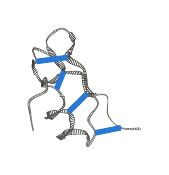
\begin{tikzpicture}[x=1pt,y=1pt]
\definecolor{s0}{rgb}{0.42,0.42,0.40}
\definecolor{s1}{rgb}{0.40,0.39,0.38}
\definecolor{s2}{rgb}{0.44,0.44,0.42}
\definecolor{s3}{rgb}{0.37,0.36,0.35}
\definecolor{s4}{rgb}{0.46,0.45,0.43}
\definecolor{s5}{rgb}{0.35,0.34,0.33}
\definecolor{s6}{rgb}{0.46,0.46,0.44}
\definecolor{s7}{rgb}{0.34,0.34,0.33}
\definecolor{s8}{rgb}{0.47,0.46,0.44}
\definecolor{s9}{rgb}{0.36,0.36,0.35}
\definecolor{s10}{rgb}{0.47,0.47,0.45}
\definecolor{s11}{rgb}{0.38,0.38,0.37}
\definecolor{s12}{rgb}{0.41,0.40,0.39}
\definecolor{s13}{rgb}{0.43,0.43,0.41}
\definecolor{s14}{rgb}{0.47,0.47,0.44}
\definecolor{s15}{rgb}{0.37,0.37,0.35}
\definecolor{s16}{rgb}{0.34,0.33,0.32}
\definecolor{s17}{rgb}{0.38,0.38,0.36}
\definecolor{s18}{rgb}{0.39,0.38,0.37}
\definecolor{s19}{rgb}{0.45,0.45,0.43}
\definecolor{s20}{rgb}{0.37,0.37,0.36}
\definecolor{s21}{rgb}{0.45,0.44,0.42}
\definecolor{s22}{rgb}{0.36,0.35,0.34}
\definecolor{s23}{rgb}{0.40,0.40,0.38}
\definecolor{s24}{rgb}{0.42,0.41,0.40}
\definecolor{s25}{rgb}{0.36,0.36,0.34}
\definecolor{s26}{rgb}{0.41,0.41,0.39}
\definecolor{s27}{rgb}{0.39,0.39,0.37}
\definecolor{s28}{rgb}{0.38,0.37,0.36}
\definecolor{s29}{rgb}{0.27,0.27,0.26}
\definecolor{s30}{rgb}{0.28,0.28,0.27}
\definecolor{s31}{rgb}{0.26,0.26,0.25}
\definecolor{s32}{rgb}{0.29,0.29,0.28}
\definecolor{s33}{rgb}{0.30,0.30,0.29}
\definecolor{s34}{rgb}{0.31,0.31,0.30}
\definecolor{s35}{rgb}{0.28,0.28,0.26}
\definecolor{s36}{rgb}{0.33,0.32,0.31}
\definecolor{s37}{rgb}{0.34,0.34,0.32}
\definecolor{s38}{rgb}{0.28,0.27,0.26}
\definecolor{s39}{rgb}{0.35,0.35,0.33}
\definecolor{s40}{rgb}{0.25,0.25,0.23}
\definecolor{s41}{rgb}{0.25,0.25,0.24}
\definecolor{s42}{rgb}{0.29,0.28,0.27}
\definecolor{s43}{rgb}{0.26,0.25,0.24}
\definecolor{s44}{rgb}{0.33,0.33,0.31}
\definecolor{s45}{rgb}{0.27,0.27,0.25}
\definecolor{s46}{rgb}{0.27,0.26,0.25}
\definecolor{s47}{rgb}{0.24,0.24,0.23}
\definecolor{s48}{rgb}{0.25,0.24,0.23}
\definecolor{s49}{rgb}{0.37,0.36,0.34}
\definecolor{s50}{rgb}{0.49,0.49,0.47}
\definecolor{s51}{rgb}{0.48,0.48,0.46}
\definecolor{s52}{rgb}{0.48,0.47,0.45}
\definecolor{s53}{rgb}{0.49,0.48,0.46}
\definecolor{s54}{rgb}{0.50,0.49,0.47}
\definecolor{s55}{rgb}{0.49,0.49,0.46}
\definecolor{s56}{rgb}{0.48,0.48,0.45}
\definecolor{s57}{rgb}{0.39,0.39,0.38}
\definecolor{s58}{rgb}{0.50,0.50,0.48}
\definecolor{s59}{rgb}{0.32,0.32,0.30}
\definecolor{s60}{rgb}{0.35,0.34,0.32}
\definecolor{s61}{rgb}{0.36,0.35,0.33}
\definecolor{s62}{rgb}{0.30,0.29,0.28}
\definecolor{s63}{rgb}{0.51,0.50,0.48}
\definecolor{s64}{rgb}{0.24,0.23,0.22}
\definecolor{s65}{rgb}{0.31,0.30,0.29}
\definecolor{s66}{rgb}{0.32,0.31,0.30}
\definecolor{s67}{rgb}{0.23,0.23,0.22}
\definecolor{s68}{rgb}{0.50,0.50,0.47}
\definecolor{s69}{rgb}{0.30,0.30,0.28}
\definecolor{s70}{rgb}{0.23,0.22,0.21}
\definecolor{s71}{rgb}{0.21,0.21,0.20}
\definecolor{s72}{rgb}{0.51,0.51,0.48}
\definecolor{s73}{rgb}{0.22,0.22,0.21}
\definecolor{s74}{rgb}{0.43,0.42,0.41}
\definecolor{s75}{rgb}{0.31,0.31,0.29}
\definecolor{s76}{rgb}{0.32,0.32,0.31}
\definecolor{s77}{rgb}{0.24,0.24,0.22}
\definecolor{s78}{rgb}{0.26,0.26,0.24}
\definecolor{s79}{rgb}{0.44,0.43,0.41}
\definecolor{s80}{rgb}{0.35,0.35,0.34}
\definecolor{s81}{rgb}{0.45,0.44,0.43}
\definecolor{s82}{rgb}{0.42,0.41,0.39}
\definecolor{s83}{rgb}{0.43,0.42,0.40}
\definecolor{s84}{rgb}{0.44,0.43,0.42}
\definecolor{s85}{rgb}{0.29,0.29,0.27}
\definecolor{s86}{rgb}{0.16,0.47,0.84}
\draw[s0,line width=0.15pt] (30.907,35.794) -- (31.342,35.727) -- (31.298,36.26) -- (30.848,36.169) -- (30.907,35.794);
\draw[s1,line width=0.15pt] (30.848,36.169) -- (31.298,36.26) -- (31.239,36.797) -- (30.793,36.537) -- (30.848,36.169);
\draw[s2,line width=0.15pt] (30.979,35.395) -- (31.393,35.214) -- (31.342,35.727) -- (30.907,35.794) -- (30.979,35.395);
\draw[s3,line width=0.15pt] (30.793,36.537) -- (31.239,36.797) -- (31.16,37.307) -- (30.71,36.944) -- (30.793,36.537);
\draw[s4,line width=0.15pt] (31.054,34.977) -- (31.453,34.712) -- (31.393,35.214) -- (30.979,35.395) -- (31.054,34.977);
\draw[s5,line width=0.15pt] (30.71,36.944) -- (31.16,37.307) -- (31.073,37.789) -- (30.607,37.378) -- (30.71,36.944);
\draw[s6,line width=0.15pt] (31.137,34.542) -- (31.52,34.218) -- (31.453,34.712) -- (31.054,34.977) -- (31.137,34.542);
\draw[s7,line width=0.15pt] (30.607,37.378) -- (31.073,37.789) -- (30.994,38.251) -- (30.493,37.836) -- (30.607,37.378);
\draw[s8,line width=0.15pt] (31.219,34.096) -- (31.599,33.732) -- (31.52,34.218) -- (31.137,34.542) -- (31.219,34.096);
\draw[s8,line width=0.15pt] (31.306,33.638) -- (31.682,33.254) -- (31.599,33.732) -- (31.219,34.096) -- (31.306,33.638);
\draw[s9,line width=0.15pt] (30.493,37.836) -- (30.994,38.251) -- (30.927,38.693) -- (30.374,38.31) -- (30.493,37.836);
\draw[s10,line width=0.15pt] (31.393,33.175) -- (31.772,32.78) -- (31.682,33.254) -- (31.306,33.638) -- (31.393,33.175);
\draw[s11,line width=0.15pt] (30.374,38.31) -- (30.927,38.693) -- (30.88,39.112) -- (30.272,38.792) -- (30.374,38.31);
\draw[s10,line width=0.15pt] (31.48,32.709) -- (31.863,32.31) -- (31.772,32.78) -- (31.393,33.175) -- (31.48,32.709);
\draw[s12,line width=0.15pt] (30.272,38.792) -- (30.88,39.112) -- (30.852,39.515) -- (30.193,39.282) -- (30.272,38.792);
\draw[s10,line width=0.15pt] (31.567,32.235) -- (31.954,31.844) -- (31.863,32.31) -- (31.48,32.709) -- (31.567,32.235);
\draw[s13,line width=0.15pt] (30.193,39.282) -- (30.852,39.515) -- (30.852,39.89) -- (30.153,39.78) -- (30.193,39.282);
\draw[s14,line width=0.15pt] (31.654,31.761) -- (32.041,31.382) -- (31.954,31.844) -- (31.567,32.235) -- (31.654,31.761);
\draw[s15,line width=0.15pt] (35.951,44.729) -- (36.354,44.172) -- (36.769,44.507) -- (36.338,45.013) -- (35.951,44.729);
\draw[s16,line width=0.15pt] (36.338,45.013) -- (36.769,44.507) -- (37.065,44.859) -- (36.627,45.321) -- (36.338,45.013);
\draw[s17,line width=0.15pt] (35.481,44.452) -- (35.853,43.856) -- (36.354,44.172) -- (35.951,44.729) -- (35.481,44.452);
\draw[s17,line width=0.15pt] (34.948,44.184) -- (35.284,43.556) -- (35.853,43.856) -- (35.481,44.452) -- (34.948,44.184);
\draw[s18,line width=0.15pt] (36.627,45.321) -- (37.065,44.859) -- (37.251,45.234) -- (36.828,45.669) -- (36.627,45.321);
\draw[s19,line width=0.15pt] (30.153,39.78) -- (30.852,39.89) -- (30.88,40.25) -- (30.169,40.269) -- (30.153,39.78);
\draw[s17,line width=0.15pt] (34.368,43.915) -- (34.676,43.271) -- (35.284,43.556) -- (34.948,44.184) -- (34.368,43.915);
\draw[s8,line width=0.15pt] (31.737,31.283) -- (32.128,30.924) -- (32.041,31.382) -- (31.654,31.761) -- (31.737,31.283);
\draw[s0,line width=0.15pt] (36.828,45.669) -- (37.251,45.234) -- (37.354,45.637) -- (36.974,46.068) -- (36.828,45.669);
\draw[s20,line width=0.15pt] (33.759,43.642) -- (34.048,42.987) -- (34.676,43.271) -- (34.368,43.915) -- (33.759,43.642);
\draw[s6,line width=0.15pt] (30.169,40.269) -- (30.88,40.25) -- (30.947,40.597) -- (30.248,40.747) -- (30.169,40.269);
\draw[s2,line width=0.15pt] (36.974,46.068) -- (37.354,45.637) -- (37.377,46.06) -- (37.077,46.51) -- (36.974,46.068);
\draw[s6,line width=0.15pt] (31.82,30.809) -- (32.207,30.466) -- (32.128,30.924) -- (31.737,31.283) -- (31.82,30.809);
\draw[s15,line width=0.15pt] (33.139,43.362) -- (33.431,42.71) -- (34.048,42.987) -- (33.759,43.642) -- (33.139,43.362);
\draw[s9,line width=0.15pt] (32.535,43.07) -- (32.843,42.426) -- (33.431,42.71) -- (33.139,43.362) -- (32.535,43.07);
\draw[s6,line width=0.15pt] (30.248,40.747) -- (30.947,40.597) -- (31.058,40.933) -- (30.402,41.209) -- (30.248,40.747);
\draw[s21,line width=0.15pt] (37.077,46.51) -- (37.377,46.06) -- (37.322,46.486) -- (37.152,46.98) -- (37.077,46.51);
\draw[s22,line width=0.15pt] (31.958,42.762) -- (32.306,42.142) -- (32.843,42.426) -- (32.535,43.07) -- (31.958,42.762);
\draw[s2,line width=0.15pt] (30.402,41.209) -- (31.058,40.933) -- (31.227,41.249) -- (30.635,41.648) -- (30.402,41.209);
\draw[s7,line width=0.15pt] (31.437,42.43) -- (31.844,41.845) -- (32.306,42.142) -- (31.958,42.762) -- (31.437,42.43);
\draw[s23,line width=0.15pt] (30.635,41.648) -- (31.227,41.249) -- (31.484,41.549) -- (30.983,42.063) -- (30.635,41.648);
\draw[s22,line width=0.15pt] (30.983,42.063) -- (31.484,41.549) -- (31.844,41.845) -- (31.437,42.43) -- (30.983,42.063);
\draw[s2,line width=0.15pt] (37.152,46.98) -- (37.322,46.486) -- (37.203,46.921) -- (37.207,47.45) -- (37.152,46.98);
\draw[s24,line width=0.15pt] (37.207,47.45) -- (37.203,46.921) -- (37.042,47.363) -- (37.235,47.908) -- (37.207,47.45);
\draw[s17,line width=0.15pt] (37.235,47.908) -- (37.042,47.363) -- (36.868,47.806) -- (37.219,48.331) -- (37.235,47.908);
\draw[s7,line width=0.15pt] (37.219,48.331) -- (36.868,47.806) -- (36.702,48.228) -- (37.16,48.718) -- (37.219,48.331);
\draw[s25,line width=0.15pt] (37.16,48.718) -- (36.702,48.228) -- (36.548,48.611) -- (37.073,49.07) -- (37.16,48.718);
\draw[s18,line width=0.15pt] (37.073,49.07) -- (36.548,48.611) -- (36.41,48.939) -- (36.967,49.374) -- (37.073,49.07);
\draw[s23,line width=0.15pt] (36.967,49.374) -- (36.41,48.939) -- (36.283,49.204) -- (36.86,49.623) -- (36.967,49.374);
\draw[s26,line width=0.15pt] (36.86,49.623) -- (36.283,49.204) -- (36.184,49.386) -- (36.761,49.804) -- (36.86,49.623);
\draw[s0,line width=0.15pt] (36.761,49.804) -- (36.184,49.386) -- (36.098,49.465) -- (36.658,49.899) -- (36.761,49.804);
\draw[s0,line width=0.15pt] (36.658,49.899) -- (36.098,49.465) -- (36.007,49.437) -- (36.54,49.887) -- (36.658,49.899);
\draw[s26,line width=0.15pt] (36.54,49.887) -- (36.007,49.437) -- (35.904,49.33) -- (36.41,49.796) -- (36.54,49.887);
\draw[s23,line width=0.15pt] (36.41,49.796) -- (35.904,49.33) -- (35.797,49.164) -- (36.271,49.642) -- (36.41,49.796);
\draw[s27,line width=0.15pt] (36.271,49.642) -- (35.797,49.164) -- (35.675,48.959) -- (36.121,49.453) -- (36.271,49.642);
\draw[s11,line width=0.15pt] (36.121,49.453) -- (35.675,48.959) -- (35.545,48.734) -- (35.967,49.243) -- (36.121,49.453);
\draw[s17,line width=0.15pt] (35.967,49.243) -- (35.545,48.734) -- (35.398,48.517) -- (35.805,49.038) -- (35.967,49.243);
\draw[s28,line width=0.15pt] (35.805,49.038) -- (35.398,48.517) -- (35.24,48.327) -- (35.643,48.86) -- (35.805,49.038);
\draw[s28,line width=0.15pt] (35.643,48.86) -- (35.24,48.327) -- (35.071,48.185) -- (35.473,48.726) -- (35.643,48.86);
\draw[s17,line width=0.15pt] (35.473,48.726) -- (35.071,48.185) -- (34.881,48.114) -- (35.308,48.663) -- (35.473,48.726);
\draw[s18,line width=0.15pt] (35.308,48.663) -- (34.881,48.114) -- (34.68,48.141) -- (35.138,48.682) -- (35.308,48.663);
\draw[s29,line width=0.15pt] (45.431,29.075) -- (45.249,31.015) -- (45.806,31.066) -- (45.964,29.127) -- (45.431,29.075);
\draw[s30,line width=0.15pt] (45.964,29.127) -- (45.806,31.066) -- (46.418,31.094) -- (46.561,29.17) -- (45.964,29.127);
\draw[s31,line width=0.15pt] (44.989,29.016) -- (44.74,30.948) -- (45.249,31.015) -- (45.431,29.075) -- (44.989,29.016);
\draw[s32,line width=0.15pt] (46.561,29.17) -- (46.418,31.094) -- (47.062,31.098) -- (47.208,29.206) -- (46.561,29.17);
\draw[s27,line width=0.15pt] (35.138,48.682) -- (34.68,48.141) -- (34.47,48.287) -- (34.96,48.805) -- (35.138,48.682);
\draw[s29,line width=0.15pt] (44.605,28.929) -- (44.25,30.829) -- (44.74,30.948) -- (44.989,29.016) -- (44.605,28.929);
\draw[s33,line width=0.15pt] (47.208,29.206) -- (47.062,31.098) -- (47.714,31.07) -- (47.888,29.23) -- (47.208,29.206);
\draw[s34,line width=0.15pt] (47.888,29.23) -- (47.714,31.07) -- (48.358,31.011) -- (48.583,29.245) -- (47.888,29.23);
\draw[s35,line width=0.15pt] (44.191,28.779) -- (43.784,30.644) -- (44.25,30.829) -- (44.605,28.929) -- (44.191,28.779);
\draw[s18,line width=0.15pt] (34.96,48.805) -- (34.47,48.287) -- (34.241,48.56) -- (34.751,49.054) -- (34.96,48.805);
\draw[s36,line width=0.15pt] (48.583,29.245) -- (48.358,31.011) -- (48.982,30.912) -- (49.274,29.253) -- (48.583,29.245);
\draw[s30,line width=0.15pt] (43.737,28.578) -- (43.369,30.414) -- (43.784,30.644) -- (44.191,28.779) -- (43.737,28.578);
\draw[s3,line width=0.15pt] (34.751,49.054) -- (34.241,48.56) -- (33.984,48.943) -- (34.49,49.405) -- (34.751,49.054);
\draw[s16,line width=0.15pt] (49.274,29.253) -- (48.982,30.912) -- (49.57,30.782) -- (49.942,29.237) -- (49.274,29.253);
\draw[s37,line width=0.15pt] (34.49,49.405) -- (33.984,48.943) -- (33.708,49.413) -- (34.198,49.844) -- (34.49,49.405);
\draw[s38,line width=0.15pt] (43.231,28.345) -- (43.029,30.15) -- (43.369,30.414) -- (43.737,28.578) -- (43.231,28.345);
\draw[s5,line width=0.15pt] (49.942,29.237) -- (49.57,30.782) -- (50.108,30.628) -- (50.562,29.198) -- (49.942,29.237);
\draw[s25,line width=0.15pt] (34.198,49.844) -- (33.708,49.413) -- (33.42,49.958) -- (33.878,50.349) -- (34.198,49.844);
\draw[s18,line width=0.15pt] (33.878,50.349) -- (33.42,49.958) -- (33.127,50.547) -- (33.542,50.898) -- (33.878,50.349);
\draw[s39,line width=0.15pt] (50.562,29.198) -- (50.108,30.628) -- (50.586,30.454) -- (51.115,29.115) -- (50.562,29.198);
\draw[s23,line width=0.15pt] (33.542,50.898) -- (33.127,50.547) -- (32.479,50.835) -- (33.57,51.811) -- (33.542,50.898);
\draw[s31,line width=0.15pt] (42.65,28.12) -- (42.808,29.838) -- (43.029,30.15) -- (43.231,28.345) -- (42.65,28.12);
\draw[s40,line width=0.15pt] (33.57,51.811) -- (32.479,50.835) -- (32.258,51.467) -- (33.187,52.391) -- (33.57,51.811);
\draw[s25,line width=0.15pt] (51.115,29.115) -- (50.586,30.454) -- (50.981,30.26) -- (51.585,28.985) -- (51.115,29.115);
\draw[s41,line width=0.15pt] (33.187,52.391) -- (32.258,51.467) -- (32.061,52.056) -- (32.827,52.988) -- (33.187,52.391);
\draw[s41,line width=0.15pt] (32.827,52.988) -- (32.061,52.056) -- (31.891,52.581) -- (32.503,53.588) -- (32.827,52.988);
\draw[s25,line width=0.15pt] (51.585,28.985) -- (50.981,30.26) -- (51.285,30.043) -- (51.948,28.807) -- (51.585,28.985);
\draw[s42,line width=0.15pt] (41.943,28.021) -- (42.777,29.391) -- (42.808,29.838) -- (42.65,28.12) -- (41.943,28.021);
\draw[s41,line width=0.15pt] (32.503,53.588) -- (31.891,52.581) -- (31.757,53.004) -- (32.223,54.181) -- (32.503,53.588);
\draw[s25,line width=0.15pt] (51.948,28.807) -- (51.285,30.043) -- (51.482,29.767) -- (52.197,28.55) -- (51.948,28.807);
\draw[s43,line width=0.15pt] (38.618,57.183) -- (40.213,57.933) -- (40.407,57.518) -- (38.937,56.637) -- (38.618,57.183);
\draw[s41,line width=0.15pt] (38.937,56.637) -- (40.407,57.518) -- (40.573,57.072) -- (39.285,56.077) -- (38.937,56.637);
\draw[s31,line width=0.15pt] (38.302,57.72) -- (39.976,58.336) -- (40.213,57.933) -- (38.618,57.183) -- (38.302,57.72);
\draw[s41,line width=0.15pt] (32.223,54.181) -- (31.757,53.004) -- (31.67,53.308) -- (31.994,54.749) -- (32.223,54.181);
\draw[s40,line width=0.15pt] (39.285,56.077) -- (40.573,57.072) -- (40.711,56.598) -- (39.66,55.512) -- (39.285,56.077);
\draw[s44,line width=0.15pt] (41.24,28.175) -- (42.82,28.708) -- (42.777,29.391) -- (41.943,28.021) -- (41.24,28.175);
\draw[s45,line width=0.15pt] (37.978,58.269) -- (39.692,58.747) -- (39.976,58.336) -- (38.302,57.72) -- (37.978,58.269);
\draw[s39,line width=0.15pt] (52.197,28.55) -- (51.482,29.767) -- (51.569,29.395) -- (52.355,28.187) -- (52.197,28.55);
\draw[s41,line width=0.15pt] (39.66,55.512) -- (40.711,56.598) -- (40.825,56.096) -- (40.075,54.955) -- (39.66,55.512);
\draw[s40,line width=0.15pt] (31.994,54.749) -- (31.67,53.308) -- (31.646,53.501) -- (31.828,55.247) -- (31.994,54.749);
\draw[s29,line width=0.15pt] (37.65,58.834) -- (39.376,59.142) -- (39.692,58.747) -- (37.978,58.269) -- (37.65,58.834);
\draw[s43,line width=0.15pt] (40.075,54.955) -- (40.825,56.096) -- (40.928,55.571) -- (40.517,54.426) -- (40.075,54.955);
\draw[s37,line width=0.15pt] (52.355,28.187) -- (51.569,29.395) -- (51.573,28.957) -- (52.434,27.74) -- (52.355,28.187);
\draw[s43,line width=0.15pt] (51.221,50.183) -- (49.665,49.694) -- (49.732,49.247) -- (51.423,49.468) -- (51.221,50.183);
\draw[s46,line width=0.15pt] (50.589,50.681) -- (49.879,50.195) -- (49.665,49.694) -- (51.221,50.183) -- (50.589,50.681);
\draw[s40,line width=0.15pt] (51.423,49.468) -- (49.732,49.247) -- (49.803,48.686) -- (51.514,48.738) -- (51.423,49.468);
\draw[s38,line width=0.15pt] (50.147,51.191) -- (49.724,50.476) -- (49.879,50.195) -- (50.589,50.681) -- (50.147,51.191);
\draw[s39,line width=0.15pt] (40.833,28.349) -- (42.662,28.056) -- (42.82,28.708) -- (41.24,28.175) -- (40.833,28.349);
\draw[s38,line width=0.15pt] (37.342,59.422) -- (39.04,59.525) -- (39.376,59.142) -- (37.65,58.834) -- (37.342,59.422);
\draw[s47,line width=0.15pt] (51.514,48.738) -- (49.803,48.686) -- (49.882,48.047) -- (51.522,48.011) -- (51.514,48.738);
\draw[s47,line width=0.15pt] (31.828,55.247) -- (31.646,53.501) -- (31.678,53.64) -- (31.749,55.607) -- (31.828,55.247);
\draw[s35,line width=0.15pt] (49.594,51.586) -- (49.487,50.653) -- (49.724,50.476) -- (50.147,51.191) -- (49.594,51.586);
\draw[s47,line width=0.15pt] (51.522,48.011) -- (49.882,48.047) -- (49.981,47.355) -- (51.478,47.292) -- (51.522,48.011);
\draw[s31,line width=0.15pt] (40.517,54.426) -- (40.928,55.571) -- (41.043,55.026) -- (40.972,53.932) -- (40.517,54.426);
\draw[s47,line width=0.15pt] (51.478,47.292) -- (49.981,47.355) -- (50.108,46.644) -- (51.407,46.601) -- (51.478,47.292);
\draw[s35,line width=0.15pt] (48.99,51.846) -- (49.144,50.772) -- (49.487,50.653) -- (49.594,51.586) -- (48.99,51.846);
\draw[s47,line width=0.15pt] (51.407,46.601) -- (50.108,46.644) -- (50.277,45.941) -- (51.332,45.945) -- (51.407,46.601);
\draw[s38,line width=0.15pt] (48.362,51.992) -- (48.694,50.851) -- (49.144,50.772) -- (48.99,51.846) -- (48.362,51.992);
\draw[s47,line width=0.15pt] (51.332,45.945) -- (50.277,45.941) -- (50.495,45.278) -- (51.281,45.333) -- (51.332,45.945);
\draw[s48,line width=0.15pt] (51.281,45.333) -- (50.495,45.278) -- (50.779,44.685) -- (51.281,44.78) -- (51.281,45.333);
\draw[s45,line width=0.15pt] (40.972,53.932) -- (41.043,55.026) -- (41.197,54.465) -- (41.414,53.485) -- (40.972,53.932);
\draw[s35,line width=0.15pt] (37.061,60.034) -- (38.689,59.88) -- (39.04,59.525) -- (37.342,59.422) -- (37.061,60.034);
\draw[s44,line width=0.15pt] (52.434,27.74) -- (51.573,28.957) -- (51.506,28.467) -- (52.458,27.247) -- (52.434,27.74);
\draw[s41,line width=0.15pt] (51.281,44.78) -- (50.779,44.685) -- (51.131,44.203) -- (51.356,44.29) -- (51.281,44.78);
\draw[s38,line width=0.15pt] (47.714,52.052) -- (48.164,50.902) -- (48.694,50.851) -- (48.362,51.992) -- (47.714,52.052);
\draw[s31,line width=0.15pt] (51.356,44.29) -- (51.131,44.203) -- (51.549,43.864) -- (51.356,44.29);
\draw[s47,line width=0.15pt] (31.749,55.607) -- (31.678,53.64) -- (31.761,53.754) -- (31.749,55.84) -- (31.749,55.607);
\draw[s45,line width=0.15pt] (51.549,43.864) -- (51.561,43.086) -- (52.367,44.128) -- (51.549,43.864);
\draw[s38,line width=0.15pt] (47.058,52.052) -- (47.572,50.93) -- (48.164,50.902) -- (47.714,52.052) -- (47.058,52.052);
\draw[s25,line width=0.15pt] (40.628,28.372) -- (42.417,27.626) -- (42.662,28.056) -- (40.833,28.349) -- (40.628,28.372);
\draw[s29,line width=0.15pt] (52.367,44.128) -- (51.561,43.086) -- (52.197,42.868) -- (52.762,44.045) -- (52.367,44.128);
\draw[s29,line width=0.15pt] (41.414,53.485) -- (41.197,54.465) -- (41.41,53.908) -- (41.837,53.079) -- (41.414,53.485);
\draw[s45,line width=0.15pt] (52.762,44.045) -- (52.197,42.868) -- (52.872,42.77) -- (53.267,44.018) -- (52.762,44.045);
\draw[s38,line width=0.15pt] (46.403,52.016) -- (46.932,50.95) -- (47.572,50.93) -- (47.058,52.052) -- (46.403,52.016);
\draw[s35,line width=0.15pt] (36.828,60.65) -- (38.329,60.228) -- (38.689,59.88) -- (37.061,60.034) -- (36.828,60.65);
\draw[s36,line width=0.15pt] (52.458,27.247) -- (51.506,28.467) -- (51.387,27.954) -- (52.43,26.721) -- (52.458,27.247);
\draw[s46,line width=0.15pt] (53.267,44.018) -- (52.872,42.77) -- (53.58,42.758) -- (53.864,44.034) -- (53.267,44.018);
\draw[s35,line width=0.15pt] (41.837,53.079) -- (41.41,53.908) -- (41.691,53.367) -- (42.232,52.719) -- (41.837,53.079);
\draw[s38,line width=0.15pt] (45.759,51.957) -- (46.268,50.981) -- (46.932,50.95) -- (46.403,52.016) -- (45.759,51.957);
\draw[s47,line width=0.15pt] (31.749,55.84) -- (31.761,53.754) -- (31.883,53.845) -- (31.824,55.978) -- (31.749,55.84);
\draw[s31,line width=0.15pt] (53.864,44.034) -- (53.58,42.758) -- (54.298,42.809) -- (54.524,44.073) -- (53.864,44.034);
\draw[s35,line width=0.15pt] (45.147,51.906) -- (45.585,51.037) -- (46.268,50.981) -- (45.759,51.957) -- (45.147,51.906);
\draw[s31,line width=0.15pt] (54.524,44.073) -- (54.298,42.809) -- (55.08,43.307) -- (55.152,43.71) -- (54.524,44.073);
\draw[s49,line width=0.15pt] (40.51,28.341) -- (42.216,27.361) -- (42.417,27.626) -- (40.628,28.372) -- (40.51,28.341);
\draw[s10,line width=0.15pt] (42.524,67.669) -- (42.571,67.187) -- (42.129,67.148) -- (42.066,67.634) -- (42.524,67.669);
\draw[s35,line width=0.15pt] (42.232,52.719) -- (41.691,53.367) -- (42.05,52.85) -- (42.599,52.415) -- (42.232,52.719);
\draw[s21,line width=0.15pt] (42.066,67.634) -- (42.129,67.148) -- (41.623,67.002) -- (41.552,67.499) -- (42.066,67.634);
\draw[s50,line width=0.15pt] (37.097,61.03) -- (37.539,60.805) -- (38.329,60.228) -- (36.828,60.65) -- (37.097,61.03);
\draw[s51,line width=0.15pt] (42.97,67.594) -- (42.982,67.112) -- (42.571,67.187) -- (42.524,67.669) -- (42.97,67.594);
\draw[s26,line width=0.15pt] (58.766,37.848) -- (58.951,37.816) -- (58.979,37.216) -- (58.789,37.188) -- (58.766,37.848);
\draw[s0,line width=0.15pt] (58.789,37.188) -- (58.979,37.216) -- (59.062,36.675) -- (58.88,36.564) -- (58.789,37.188);
\draw[s19,line width=0.15pt] (55.152,43.71) -- (55.08,43.307) -- (55.78,43.382) -- (55.855,43.765) -- (55.152,43.71);
\draw[s12,line width=0.15pt] (58.801,38.527) -- (58.967,38.46) -- (58.951,37.816) -- (58.766,37.848) -- (58.801,38.527);
\draw[s35,line width=0.15pt] (44.574,51.866) -- (44.906,51.135) -- (45.585,51.037) -- (45.147,51.906) -- (44.574,51.866);
\draw[s0,line width=0.15pt] (41.552,67.499) -- (41.623,67.002) -- (41.094,66.757) -- (40.983,67.286) -- (41.552,67.499);
\draw[s2,line width=0.15pt] (58.88,36.564) -- (59.062,36.675) -- (59.216,36.201) -- (59.07,36.0) -- (58.88,36.564);
\draw[s23,line width=0.15pt] (58.868,39.219) -- (58.999,39.132) -- (58.967,38.46) -- (58.801,38.527) -- (58.868,39.219);
\draw[s36,line width=0.15pt] (52.43,26.721) -- (51.387,27.954) -- (51.605,27.037) -- (52.015,26.587) -- (52.43,26.721);
\draw[s52,line width=0.15pt] (43.44,67.42) -- (43.405,66.931) -- (42.982,67.112) -- (42.97,67.594) -- (43.44,67.42);
\draw[s42,line width=0.15pt] (42.599,52.415) -- (42.05,52.85) -- (42.492,52.36) -- (42.935,52.178) -- (42.599,52.415);
\draw[s19,line width=0.15pt] (55.855,43.765) -- (55.78,43.382) -- (56.447,43.445) -- (56.542,43.793) -- (55.855,43.765);
\draw[s42,line width=0.15pt] (44.06,51.858) -- (44.242,51.301) -- (44.906,51.135) -- (44.574,51.866) -- (44.06,51.858);
\draw[s23,line width=0.15pt] (58.951,39.906) -- (59.038,39.807) -- (58.999,39.132) -- (58.868,39.219) -- (58.951,39.906);
\draw[s4,line width=0.15pt] (59.07,36.0) -- (59.216,36.201) -- (59.429,35.759) -- (59.33,35.486) -- (59.07,36.0);
\draw[s1,line width=0.15pt] (40.983,67.286) -- (41.094,66.757) -- (40.557,66.433) -- (40.367,67.002) -- (40.983,67.286);
\draw[s42,line width=0.15pt] (42.935,52.178) -- (42.492,52.36) -- (43.018,51.913) -- (43.255,52.004) -- (42.935,52.178);
\draw[s42,line width=0.15pt] (43.618,51.902) -- (43.606,51.554) -- (44.242,51.301) -- (44.06,51.858) -- (43.618,51.902);
\draw[s23,line width=0.15pt] (59.03,40.577) -- (59.062,40.479) -- (59.038,39.807) -- (58.951,39.906) -- (59.03,40.577);
\draw[s42,line width=0.15pt] (43.255,52.004) -- (43.018,51.913) -- (43.606,51.554) -- (43.618,51.902) -- (43.255,52.004);
\draw[s6,line width=0.15pt] (56.542,43.793) -- (56.447,43.445) -- (57.063,43.465) -- (57.19,43.773) -- (56.542,43.793);
\draw[s14,line width=0.15pt] (43.926,67.16) -- (43.839,66.658) -- (43.405,66.931) -- (43.44,67.42) -- (43.926,67.16);
\draw[s48,line width=0.15pt] (31.824,55.978) -- (31.883,53.845) -- (32.037,53.9) -- (31.954,56.057) -- (31.824,55.978);
\draw[s8,line width=0.15pt] (59.33,35.486) -- (59.429,35.759) -- (59.678,35.312) -- (59.631,35.0) -- (59.33,35.486);
\draw[s26,line width=0.15pt] (59.09,41.213) -- (59.058,41.122) -- (59.062,40.479) -- (59.03,40.577) -- (59.09,41.213);
\draw[s53,line width=0.15pt] (36.911,61.527) -- (37.29,61.247) -- (37.539,60.805) -- (37.097,61.03) -- (36.911,61.527);
\draw[s10,line width=0.15pt] (57.19,43.773) -- (57.063,43.465) -- (57.616,43.425) -- (57.77,43.682) -- (57.19,43.773);
\draw[s3,line width=0.15pt] (40.367,67.002) -- (40.557,66.433) -- (40.039,66.05) -- (39.72,66.65) -- (40.367,67.002);
\draw[s0,line width=0.15pt] (59.105,41.81) -- (59.007,41.719) -- (59.058,41.122) -- (59.09,41.213) -- (59.105,41.81);
\draw[s15,line width=0.15pt] (40.462,28.325) -- (42.089,27.211) -- (42.216,27.361) -- (40.51,28.341) -- (40.462,28.325);
\draw[s53,line width=0.15pt] (57.77,43.682) -- (57.616,43.425) -- (58.082,43.303) -- (58.272,43.5) -- (57.77,43.682);
\draw[s2,line width=0.15pt] (59.054,42.351) -- (58.896,42.256) -- (59.007,41.719) -- (59.105,41.81) -- (59.054,42.351);
\draw[s54,line width=0.15pt] (58.272,43.5) -- (58.082,43.303) -- (58.45,43.07) -- (58.655,43.212) -- (58.272,43.5);
\draw[s4,line width=0.15pt] (44.412,66.82) -- (44.27,66.311) -- (43.839,66.658) -- (43.926,67.16) -- (44.412,66.82);
\draw[s10,line width=0.15pt] (59.631,35.0) -- (59.678,35.312) -- (59.955,34.862) -- (59.97,34.534) -- (59.631,35.0);
\draw[s6,line width=0.15pt] (58.912,42.821) -- (58.714,42.71) -- (58.896,42.256) -- (59.054,42.351) -- (58.912,42.821);
\draw[s55,line width=0.15pt] (58.655,43.212) -- (58.45,43.07) -- (58.714,42.71) -- (58.912,42.821) -- (58.655,43.212);
\draw[s2,line width=0.15pt] (52.015,26.587) -- (51.605,27.037) -- (51.474,26.528) -- (51.921,26.082) -- (52.015,26.587);
\draw[s7,line width=0.15pt] (39.72,66.65) -- (40.039,66.05) -- (39.53,65.663) -- (39.076,66.208) -- (39.72,66.65);
\draw[s10,line width=0.15pt] (36.773,62.005) -- (37.105,61.693) -- (37.29,61.247) -- (36.911,61.527) -- (36.773,62.005);
\draw[s56,line width=0.15pt] (59.97,34.534) -- (59.955,34.862) -- (60.259,34.42) -- (60.346,34.1) -- (59.97,34.534);
\draw[s2,line width=0.15pt] (44.886,66.413) -- (44.692,65.9) -- (44.27,66.311) -- (44.412,66.82) -- (44.886,66.413);
\draw[s48,line width=0.15pt] (31.954,56.057) -- (32.037,53.9) -- (32.211,53.932) -- (32.12,56.092) -- (31.954,56.057);
\draw[s18,line width=0.15pt] (39.076,66.208) -- (39.53,65.663) -- (38.993,65.295) -- (38.507,65.675) -- (39.076,66.208);
\draw[s15,line width=0.15pt] (40.494,28.372) -- (42.05,27.16) -- (42.089,27.211) -- (40.462,28.325) -- (40.494,28.372);
\draw[s53,line width=0.15pt] (60.346,34.1) -- (60.259,34.42) -- (60.587,33.977) -- (60.752,33.693) -- (60.346,34.1);
\draw[s19,line width=0.15pt] (36.698,62.456) -- (36.994,62.144) -- (37.105,61.693) -- (36.773,62.005) -- (36.698,62.456);
\draw[s13,line width=0.15pt] (45.344,65.959) -- (45.099,65.45) -- (44.692,65.9) -- (44.886,66.413) -- (45.344,65.959);
\draw[s21,line width=0.15pt] (51.921,26.082) -- (51.474,26.528) -- (51.348,26.066) -- (51.826,25.619) -- (51.921,26.082);
\draw[s26,line width=0.15pt] (38.507,65.675) -- (38.993,65.295) -- (38.46,64.893) -- (38.013,65.13) -- (38.507,65.675);
\draw[s54,line width=0.15pt] (60.752,33.693) -- (60.587,33.977) -- (60.942,33.547) -- (61.183,33.314) -- (60.752,33.693);
\draw[s12,line width=0.15pt] (38.013,65.13) -- (38.46,64.893) -- (37.982,64.446) -- (37.579,64.608) -- (38.013,65.13);
\draw[s0,line width=0.15pt] (36.686,62.874) -- (36.982,62.598) -- (36.994,62.144) -- (36.698,62.456) -- (36.686,62.874);
\draw[s25,line width=0.15pt] (40.656,28.479) -- (42.117,27.191) -- (42.05,27.16) -- (40.494,28.372) -- (40.656,28.479);
\draw[s40,line width=0.15pt] (46.063,65.971) -- (45.19,64.454) -- (45.099,65.45) -- (45.344,65.959) -- (46.063,65.971);
\draw[s57,line width=0.15pt] (37.579,64.608) -- (37.982,64.446) -- (37.579,63.976) -- (37.215,64.118) -- (37.579,64.608);
\draw[s48,line width=0.15pt] (32.12,56.092) -- (32.211,53.932) -- (32.4,53.952) -- (32.318,56.112) -- (32.12,56.092);
\draw[s28,line width=0.15pt] (36.761,63.265) -- (37.069,63.048) -- (36.982,62.598) -- (36.686,62.874) -- (36.761,63.265);
\draw[s20,line width=0.15pt] (37.215,64.118) -- (37.579,63.976) -- (37.271,63.506) -- (36.935,63.668) -- (37.215,64.118);
\draw[s4,line width=0.15pt] (51.826,25.619) -- (51.348,26.066) -- (51.245,25.663) -- (51.751,25.224) -- (51.826,25.619);
\draw[s7,line width=0.15pt] (36.935,63.668) -- (37.271,63.506) -- (37.069,63.048) -- (36.761,63.265) -- (36.935,63.668);
\draw[s58,line width=0.15pt] (61.183,33.314) -- (60.942,33.547) -- (61.329,33.132) -- (61.629,32.97) -- (61.183,33.314);
\draw[s5,line width=0.15pt] (41.296,37.109) -- (41.138,37.508) -- (41.999,37.129) -- (41.896,37.745) -- (41.296,37.109);
\draw[s47,line width=0.15pt] (46.486,65.442) -- (45.502,63.964) -- (45.19,64.454) -- (46.063,65.971) -- (46.486,65.442);
\draw[s39,line width=0.15pt] (41.896,37.745) -- (41.999,37.129) -- (42.745,36.979) -- (42.567,38.073) -- (41.896,37.745);
\draw[s59,line width=0.15pt] (40.715,36.462) -- (40.273,37.856) -- (41.138,37.508) -- (41.296,37.109) -- (40.715,36.462);
\draw[s60,line width=0.15pt] (42.567,38.073) -- (42.745,36.979) -- (43.401,36.916) -- (43.247,38.215) -- (42.567,38.073);
\draw[s61,line width=0.15pt] (40.952,28.633) -- (42.307,27.274) -- (42.117,27.191) -- (40.656,28.479) -- (40.952,28.633);
\draw[s37,line width=0.15pt] (43.247,38.215) -- (43.401,36.916) -- (43.954,36.853) -- (43.898,38.235) -- (43.247,38.215);
\draw[s62,line width=0.15pt] (40.079,36.114) -- (39.518,37.868) -- (40.273,37.856) -- (40.715,36.462) -- (40.079,36.114);
\draw[s37,line width=0.15pt] (43.898,38.235) -- (43.954,36.853) -- (44.38,36.762) -- (44.499,38.14) -- (43.898,38.235);
\draw[s63,line width=0.15pt] (61.629,32.97) -- (61.329,33.132) -- (61.74,32.737) -- (62.087,32.654) -- (61.629,32.97);
\draw[s42,line width=0.15pt] (39.455,35.897) -- (38.858,37.745) -- (39.518,37.868) -- (40.079,36.114) -- (39.455,35.897);
\draw[s5,line width=0.15pt] (44.499,38.14) -- (44.38,36.762) -- (44.673,36.608) -- (45.012,37.935) -- (44.499,38.14);
\draw[s47,line width=0.15pt] (46.849,64.897) -- (45.775,63.475) -- (45.502,63.964) -- (46.486,65.442) -- (46.849,64.897);
\draw[s42,line width=0.15pt] (38.89,35.719) -- (38.286,37.595) -- (38.858,37.745) -- (39.455,35.897) -- (38.89,35.719);
\draw[s14,line width=0.15pt] (51.751,25.224) -- (51.245,25.663) -- (51.186,25.351) -- (51.711,24.916) -- (51.751,25.224);
\draw[s37,line width=0.15pt] (45.012,37.935) -- (44.673,36.608) -- (44.898,36.343) -- (45.415,37.635) -- (45.012,37.935);
\draw[s48,line width=0.15pt] (32.318,56.112) -- (32.4,53.952) -- (32.566,54.686) -- (32.547,55.401) -- (32.318,56.112);
\draw[s63,line width=0.15pt] (62.087,32.654) -- (61.74,32.737) -- (62.178,32.37) -- (62.55,32.37) -- (62.087,32.654);
\draw[s5,line width=0.15pt] (41.351,28.846) -- (42.603,27.397) -- (42.307,27.274) -- (40.952,28.633) -- (41.351,28.846);
\draw[s32,line width=0.15pt] (38.416,35.573) -- (37.824,37.457) -- (38.286,37.595) -- (38.89,35.719) -- (38.416,35.573);
\draw[s44,line width=0.15pt] (45.415,37.635) -- (44.898,36.343) -- (45.083,35.968) -- (45.767,37.24) -- (45.415,37.635);
\draw[s64,line width=0.15pt] (47.149,64.348) -- (46.004,62.997) -- (45.775,63.475) -- (46.849,64.897) -- (47.149,64.348);
\draw[s58,line width=0.15pt] (62.55,32.37) -- (62.178,32.37) -- (62.64,32.038) -- (63.016,32.113) -- (62.55,32.37);
\draw[s65,line width=0.15pt] (38.069,35.466) -- (37.484,37.346) -- (37.824,37.457) -- (38.416,35.573) -- (38.069,35.466);
\draw[s51,line width=0.15pt] (51.711,24.916) -- (51.186,25.351) -- (51.182,25.149) -- (51.727,24.723) -- (51.711,24.916);
\draw[s66,line width=0.15pt] (45.767,37.24) -- (45.083,35.968) -- (45.19,35.53) -- (46.114,36.742) -- (45.767,37.24);
\draw[s16,line width=0.15pt] (41.845,29.127) -- (42.962,27.535) -- (42.603,27.397) -- (41.351,28.846) -- (41.845,29.127);
\draw[s67,line width=0.15pt] (47.374,63.814) -- (46.178,62.55) -- (46.004,62.997) -- (47.149,64.348) -- (47.374,63.814);
\draw[s68,line width=0.15pt] (63.016,32.113) -- (62.64,32.038) -- (63.126,31.738) -- (63.482,31.888) -- (63.016,32.113);
\draw[s26,line width=0.15pt] (32.547,55.401) -- (32.566,54.686) -- (32.752,54.706) -- (32.74,55.421) -- (32.547,55.401);
\draw[s59,line width=0.15pt] (37.835,35.364) -- (37.231,37.224) -- (37.484,37.346) -- (38.069,35.466) -- (37.835,35.364);
\draw[s69,line width=0.15pt] (46.114,36.742) -- (45.19,35.53) -- (45.194,35.067) -- (46.478,36.134) -- (46.114,36.742);
\draw[s50,line width=0.15pt] (63.482,31.888) -- (63.126,31.738) -- (63.628,31.477) -- (63.948,31.694) -- (63.482,31.888);
\draw[s58,line width=0.15pt] (51.727,24.723) -- (51.182,25.149) -- (51.257,25.086) -- (51.81,24.66) -- (51.727,24.723);
\draw[s70,line width=0.15pt] (46.9,62.728) -- (46.178,62.55) -- (47.374,63.814) -- (46.9,62.728);
\draw[s66,line width=0.15pt] (42.453,29.463) -- (43.326,27.693) -- (42.962,27.535) -- (41.845,29.127) -- (42.453,29.463);
\draw[s55,line width=0.15pt] (63.948,31.694) -- (63.628,31.477) -- (64.149,31.268) -- (64.426,31.544) -- (63.948,31.694);
\draw[s29,line width=0.15pt] (46.478,36.134) -- (45.194,35.067) -- (45.107,34.653) -- (46.849,35.375) -- (46.478,36.134);
\draw[s59,line width=0.15pt] (37.654,35.221) -- (37.073,37.066) -- (37.231,37.224) -- (37.835,35.364) -- (37.654,35.221);
\draw[s51,line width=0.15pt] (64.426,31.544) -- (64.149,31.268) -- (64.702,31.11) -- (64.931,31.445) -- (64.426,31.544);
\draw[s71,line width=0.15pt] (47.019,62.353) -- (46.809,62.207) -- (46.9,62.728) -- (47.019,62.353);
\draw[s26,line width=0.15pt] (32.74,55.421) -- (32.752,54.706) -- (32.922,54.753) -- (32.922,55.464) -- (32.74,55.421);
\draw[s72,line width=0.15pt] (51.81,24.66) -- (51.257,25.086) -- (51.415,25.165) -- (51.968,24.735) -- (51.81,24.66);
\draw[s10,line width=0.15pt] (64.931,31.445) -- (64.702,31.11) -- (65.279,30.995) -- (65.461,31.386) -- (64.931,31.445);
\draw[s29,line width=0.15pt] (43.243,29.731) -- (43.571,27.985) -- (43.326,27.693) -- (42.453,29.463) -- (43.243,29.731);
\draw[s6,line width=0.15pt] (65.461,31.386) -- (65.279,30.995) -- (65.875,30.92) -- (66.018,31.358) -- (65.461,31.386);
\draw[s73,line width=0.15pt] (47.019,61.918) -- (46.588,61.701) -- (46.809,62.207) -- (47.019,62.353) -- (47.019,61.918);
\draw[s38,line width=0.15pt] (46.849,35.375) -- (45.107,34.653) -- (45.099,34.341) -- (47.058,34.455) -- (46.849,35.375);
\draw[s19,line width=0.15pt] (66.018,31.358) -- (65.875,30.92) -- (66.484,30.873) -- (66.59,31.358) -- (66.018,31.358);
\draw[s54,line width=0.15pt] (51.968,24.735) -- (51.415,25.165) -- (51.636,25.359) -- (52.193,24.92) -- (51.968,24.735);
\draw[s59,line width=0.15pt] (37.476,35.04) -- (37.026,36.896) -- (37.073,37.066) -- (37.654,35.221) -- (37.476,35.04);
\draw[s2,line width=0.15pt] (66.59,31.358) -- (66.484,30.873) -- (67.1,30.849) -- (67.179,31.378) -- (66.59,31.358);
\draw[s74,line width=0.15pt] (67.179,31.378) -- (67.1,30.849) -- (67.724,30.841) -- (67.779,31.41) -- (67.179,31.378);
\draw[s62,line width=0.15pt] (44.128,29.739) -- (43.737,28.598) -- (43.571,27.985) -- (43.243,29.731) -- (44.128,29.739);
\draw[s12,line width=0.15pt] (32.922,55.464) -- (32.922,54.753) -- (33.06,54.844) -- (33.072,55.547) -- (32.922,55.464);
\draw[s67,line width=0.15pt] (46.924,61.44) -- (46.268,61.211) -- (46.588,61.701) -- (47.019,61.918) -- (46.924,61.44);
\draw[s26,line width=0.15pt] (67.779,31.41) -- (67.724,30.841) -- (68.348,30.841) -- (68.387,31.445) -- (67.779,31.41);
\draw[s75,line width=0.15pt] (47.058,34.455) -- (45.099,34.341) -- (45.281,33.965) -- (46.999,33.566) -- (47.058,34.455);
\draw[s23,line width=0.15pt] (68.387,31.445) -- (68.348,30.841) -- (68.964,30.845) -- (69.0,31.481) -- (68.387,31.445);
\draw[s52,line width=0.15pt] (52.193,24.92) -- (51.636,25.359) -- (51.913,25.647) -- (52.47,25.205) -- (52.193,24.92);
\draw[s27,line width=0.15pt] (69.0,31.481) -- (68.964,30.845) -- (69.572,30.841) -- (69.616,31.505) -- (69.0,31.481);
\draw[s66,line width=0.15pt] (44.835,29.759) -- (44.056,29.249) -- (43.737,28.598) -- (44.128,29.739) -- (44.835,29.759);
\draw[s64,line width=0.15pt] (46.762,60.931) -- (45.869,60.726) -- (46.268,61.211) -- (46.924,61.44) -- (46.762,60.931);
\draw[s28,line width=0.15pt] (69.616,31.505) -- (69.572,30.841) -- (70.169,30.833) -- (70.224,31.513) -- (69.616,31.505);
\draw[s76,line width=0.15pt] (46.999,33.566) -- (45.281,33.965) -- (45.455,33.456) -- (46.869,32.824) -- (46.999,33.566);
\draw[s75,line width=0.15pt] (37.259,34.834) -- (37.132,36.726) -- (37.026,36.896) -- (37.476,35.04) -- (37.259,34.834);
\draw[s9,line width=0.15pt] (70.224,31.513) -- (70.169,30.833) -- (70.757,30.802) -- (70.817,31.497) -- (70.224,31.513);
\draw[s4,line width=0.15pt] (52.47,25.205) -- (51.913,25.647) -- (52.225,26.018) -- (52.778,25.572) -- (52.47,25.205);
\draw[s23,line width=0.15pt] (33.072,55.547) -- (33.06,54.844) -- (33.155,54.99) -- (33.183,55.67) -- (33.072,55.547);
\draw[s59,line width=0.15pt] (45.384,29.929) -- (44.451,29.794) -- (44.056,29.249) -- (44.835,29.759) -- (45.384,29.929);
\draw[s47,line width=0.15pt] (46.561,60.406) -- (45.423,60.24) -- (45.869,60.726) -- (46.762,60.931) -- (46.561,60.406);
\draw[s59,line width=0.15pt] (46.869,32.824) -- (45.455,33.456) -- (45.534,32.879) -- (46.75,32.184) -- (46.869,32.824);
\draw[s75,line width=0.15pt] (45.83,30.193) -- (44.827,30.272) -- (44.451,29.794) -- (45.384,29.929) -- (45.83,30.193);
\draw[s2,line width=0.15pt] (52.778,25.572) -- (52.225,26.018) -- (52.556,26.457) -- (53.109,26.006) -- (52.778,25.572);
\draw[s34,line width=0.15pt] (46.75,32.184) -- (45.534,32.879) -- (45.53,32.287) -- (46.644,31.639) -- (46.75,32.184);
\draw[s47,line width=0.15pt] (46.347,59.88) -- (44.941,59.754) -- (45.423,60.24) -- (46.561,60.406) -- (46.347,59.88);
\draw[s29,line width=0.15pt] (36.868,34.688) -- (37.519,36.489) -- (37.132,36.726) -- (37.259,34.834) -- (36.868,34.688);
\draw[s32,line width=0.15pt] (46.178,30.517) -- (45.123,30.719) -- (44.827,30.272) -- (45.83,30.193) -- (46.178,30.517);
\draw[s23,line width=0.15pt] (33.183,55.67) -- (33.155,54.99) -- (33.198,55.212) -- (33.234,55.855) -- (33.183,55.67);
\draw[s33,line width=0.15pt] (46.644,31.639) -- (45.53,32.287) -- (45.447,31.71) -- (46.537,31.193) -- (46.644,31.639);
\draw[s31,line width=0.15pt] (46.403,30.845) -- (45.32,31.181) -- (45.123,30.719) -- (46.178,30.517) -- (46.403,30.845);
\draw[s30,line width=0.15pt] (46.537,31.193) -- (45.447,31.71) -- (45.32,31.181) -- (46.403,30.845) -- (46.537,31.193);
\draw[s13,line width=0.15pt] (53.109,26.006) -- (52.556,26.457) -- (52.9,26.939) -- (53.445,26.492) -- (53.109,26.006);
\draw[s47,line width=0.15pt] (46.146,59.367) -- (44.459,59.26) -- (44.941,59.754) -- (46.347,59.88) -- (46.146,59.367);
\draw[s23,line width=0.15pt] (33.234,55.855) -- (33.198,55.212) -- (33.175,55.516) -- (33.218,56.12) -- (33.234,55.855);
\draw[s74,line width=0.15pt] (53.445,26.492) -- (52.9,26.939) -- (53.232,27.448) -- (53.773,27.01) -- (53.445,26.492);
\draw[s77,line width=0.15pt] (45.988,58.893) -- (43.993,58.739) -- (44.459,59.26) -- (46.146,59.367) -- (45.988,58.893);
\draw[s59,line width=0.15pt] (36.374,34.933) -- (38.108,35.877) -- (37.519,36.489) -- (36.868,34.688) -- (36.374,34.933);
\draw[s0,line width=0.15pt] (53.773,27.01) -- (53.232,27.448) -- (53.544,27.977) -- (54.077,27.551) -- (53.773,27.01);
\draw[s67,line width=0.15pt] (45.889,58.486) -- (43.579,58.17) -- (43.993,58.739) -- (45.988,58.893) -- (45.889,58.486);
\draw[s26,line width=0.15pt] (33.218,56.12) -- (33.175,55.516) -- (33.08,55.899) -- (33.135,56.464) -- (33.218,56.12);
\draw[s70,line width=0.15pt] (45.869,58.194) -- (43.251,57.526) -- (43.579,58.17) -- (45.889,58.486) -- (45.869,58.194);
\draw[s0,line width=0.15pt] (54.077,27.551) -- (53.544,27.977) -- (53.813,28.503) -- (54.346,28.092) -- (54.077,27.551);
\draw[s25,line width=0.15pt] (36.354,35.265) -- (38.302,35.217) -- (38.108,35.877) -- (36.374,34.933) -- (36.354,35.265);
\draw[s71,line width=0.15pt] (45.281,57.767) -- (43.701,57.056) -- (43.251,57.526) -- (45.869,58.194) -- (45.281,57.767);
\draw[s24,line width=0.15pt] (33.135,56.464) -- (33.08,55.899) -- (32.93,56.333) -- (33.001,56.87) -- (33.135,56.464);
\draw[s13,line width=0.15pt] (54.346,28.092) -- (53.813,28.503) -- (54.034,29.008) -- (54.563,28.617) -- (54.346,28.092);
\draw[s67,line width=0.15pt] (45.293,57.534) -- (43.819,56.444) -- (43.701,57.056) -- (45.281,57.767) -- (45.293,57.534);
\draw[s77,line width=0.15pt] (45.403,57.313) -- (44.12,55.887) -- (43.819,56.444) -- (45.293,57.534) -- (45.403,57.313);
\draw[s2,line width=0.15pt] (54.563,28.617) -- (54.034,29.008) -- (54.18,29.482) -- (54.713,29.111) -- (54.563,28.617);
\draw[s0,line width=0.15pt] (33.001,56.87) -- (32.93,56.333) -- (32.748,56.807) -- (32.839,57.325) -- (33.001,56.87);
\draw[s15,line width=0.15pt] (36.524,35.352) -- (38.381,34.862) -- (38.302,35.217) -- (36.354,35.265) -- (36.524,35.352);
\draw[s47,line width=0.15pt] (45.625,57.068) -- (44.55,55.429) -- (44.12,55.887) -- (45.403,57.313) -- (45.625,57.068);
\draw[s48,line width=0.15pt] (45.96,56.795) -- (45.068,55.054) -- (44.55,55.429) -- (45.625,57.068) -- (45.96,56.795);
\draw[s19,line width=0.15pt] (54.713,29.111) -- (54.18,29.482) -- (54.247,29.901) -- (54.784,29.565) -- (54.713,29.111);
\draw[s41,line width=0.15pt] (46.395,56.499) -- (45.64,54.738) -- (45.068,55.054) -- (45.96,56.795) -- (46.395,56.499);
\draw[s0,line width=0.15pt] (32.839,57.325) -- (32.748,56.807) -- (32.547,57.301) -- (32.657,57.807) -- (32.839,57.325);
\draw[s43,line width=0.15pt] (46.9,56.183) -- (46.253,54.469) -- (45.64,54.738) -- (46.395,56.499) -- (46.9,56.183);
\draw[s78,line width=0.15pt] (51.806,46.719) -- (50.953,46.368) -- (50.791,47.039) -- (51.699,47.189) -- (51.806,46.719);
\draw[s43,line width=0.15pt] (51.699,47.189) -- (50.791,47.039) -- (50.68,47.711) -- (51.628,47.711) -- (51.699,47.189);
\draw[s31,line width=0.15pt] (51.952,46.297) -- (51.178,45.708) -- (50.953,46.368) -- (51.806,46.719) -- (51.952,46.297);
\draw[s41,line width=0.15pt] (51.628,47.711) -- (50.68,47.711) -- (50.609,48.378) -- (51.577,48.268) -- (51.628,47.711);
\draw[s46,line width=0.15pt] (52.169,45.894) -- (51.478,45.084) -- (51.178,45.708) -- (51.952,46.297) -- (52.169,45.894);
\draw[s41,line width=0.15pt] (51.577,48.268) -- (50.609,48.378) -- (50.566,49.03) -- (51.533,48.856) -- (51.577,48.268);
\draw[s31,line width=0.15pt] (47.453,55.844) -- (46.881,54.232) -- (46.253,54.469) -- (46.9,56.183) -- (47.453,55.844);
\draw[s10,line width=0.15pt] (54.784,29.565) -- (54.247,29.901) -- (54.211,30.276) -- (54.757,29.996) -- (54.784,29.565);
\draw[s15,line width=0.15pt] (36.722,35.352) -- (38.495,34.676) -- (38.381,34.862) -- (36.524,35.352) -- (36.722,35.352);
\draw[s41,line width=0.15pt] (51.533,48.856) -- (50.566,49.03) -- (50.53,49.666) -- (51.494,49.468) -- (51.533,48.856);
\draw[s45,line width=0.15pt] (48.034,55.472) -- (47.513,54.015) -- (46.881,54.232) -- (47.453,55.844) -- (48.034,55.472);
\draw[s45,line width=0.15pt] (52.47,45.483) -- (51.834,44.504) -- (51.478,45.084) -- (52.169,45.894) -- (52.47,45.483);
\draw[s41,line width=0.15pt] (51.494,49.468) -- (50.53,49.666) -- (50.499,50.274) -- (51.439,50.093) -- (51.494,49.468);
\draw[s38,line width=0.15pt] (48.615,55.073) -- (48.125,53.805) -- (47.513,54.015) -- (48.034,55.472) -- (48.615,55.073);
\draw[s41,line width=0.15pt] (51.439,50.093) -- (50.499,50.274) -- (50.459,50.855) -- (51.36,50.725) -- (51.439,50.093);
\draw[s45,line width=0.15pt] (52.829,45.064) -- (52.237,43.958) -- (51.834,44.504) -- (52.47,45.483) -- (52.829,45.064);
\draw[s35,line width=0.15pt] (49.175,54.647) -- (48.698,53.58) -- (48.125,53.805) -- (48.615,55.073) -- (49.175,54.647);
\draw[s24,line width=0.15pt] (32.657,57.807) -- (32.547,57.301) -- (32.341,57.795) -- (32.476,58.3) -- (32.657,57.807);
\draw[s79,line width=0.15pt] (40.332,45.301) -- (40.746,45.752) -- (41.09,45.42) -- (40.679,44.942) -- (40.332,45.301);
\draw[s19,line width=0.15pt] (39.953,45.602) -- (40.348,46.036) -- (40.746,45.752) -- (40.332,45.301) -- (39.953,45.602);
\draw[s35,line width=0.15pt] (49.693,54.192) -- (49.207,53.324) -- (48.698,53.58) -- (49.175,54.647) -- (49.693,54.192);
\draw[s43,line width=0.15pt] (51.36,50.725) -- (50.459,50.855) -- (50.392,51.392) -- (51.237,51.357) -- (51.36,50.725);
\draw[s35,line width=0.15pt] (50.147,53.711) -- (49.634,53.027) -- (49.207,53.324) -- (49.693,54.192) -- (50.147,53.711);
\draw[s26,line width=0.15pt] (40.679,44.942) -- (41.09,45.42) -- (41.446,45.041) -- (41.031,44.539) -- (40.679,44.942);
\draw[s78,line width=0.15pt] (51.237,51.357) -- (50.392,51.392) -- (50.297,51.882) -- (51.067,51.981) -- (51.237,51.357);
\draw[s38,line width=0.15pt] (50.53,53.181) -- (49.95,52.692) -- (49.634,53.027) -- (50.147,53.711) -- (50.53,53.181);
\draw[s45,line width=0.15pt] (53.236,44.642) -- (52.663,43.441) -- (52.237,43.958) -- (52.829,45.064) -- (53.236,44.642);
\draw[s31,line width=0.15pt] (51.067,51.981) -- (50.297,51.882) -- (50.155,52.316) -- (50.83,52.593) -- (51.067,51.981);
\draw[s45,line width=0.15pt] (50.83,52.593) -- (50.155,52.316) -- (49.95,52.692) -- (50.53,53.181) -- (50.83,52.593);
\draw[s6,line width=0.15pt] (39.49,45.862) -- (39.87,46.281) -- (40.348,46.036) -- (39.953,45.602) -- (39.49,45.862);
\draw[s53,line width=0.15pt] (54.757,29.996) -- (54.211,30.276) -- (54.073,30.64) -- (54.638,30.43) -- (54.757,29.996);
\draw[s27,line width=0.15pt] (41.031,44.539) -- (41.446,45.041) -- (41.817,44.602) -- (41.359,44.105) -- (41.031,44.539);
\draw[s46,line width=0.15pt] (53.666,44.215) -- (53.098,42.943) -- (52.663,43.441) -- (53.236,44.642) -- (53.666,44.215);
\draw[s10,line width=0.15pt] (38.961,46.103) -- (39.336,46.475) -- (39.87,46.281) -- (39.49,45.862) -- (38.961,46.103);
\draw[s15,line width=0.15pt] (36.931,35.356) -- (38.649,34.597) -- (38.495,34.676) -- (36.722,35.352) -- (36.931,35.356);
\draw[s26,line width=0.15pt] (32.476,58.3) -- (32.341,57.795) -- (32.152,58.277) -- (32.314,58.782) -- (32.476,58.3);
\draw[s46,line width=0.15pt] (54.109,43.785) -- (53.524,42.469) -- (53.098,42.943) -- (53.666,44.215) -- (54.109,43.785);
\draw[s3,line width=0.15pt] (41.359,44.105) -- (41.817,44.602) -- (42.208,44.109) -- (41.659,43.658) -- (41.359,44.105);
\draw[s51,line width=0.15pt] (38.381,46.34) -- (38.772,46.613) -- (39.336,46.475) -- (38.961,46.103) -- (38.381,46.34);
\draw[s54,line width=0.15pt] (54.638,30.43) -- (54.073,30.64) -- (53.86,30.999) -- (54.441,30.861) -- (54.638,30.43);
\draw[s4,line width=0.15pt] (54.334,42.896) -- (54.132,42.458) -- (53.524,42.469) -- (54.109,43.785) -- (54.334,42.896);
\draw[s12,line width=0.15pt] (32.314,58.782) -- (32.152,58.277) -- (31.99,58.723) -- (32.179,59.236) -- (32.314,58.782);
\draw[s39,line width=0.15pt] (41.659,43.658) -- (42.208,44.109) -- (42.579,43.52) -- (41.935,43.251) -- (41.659,43.658);
\draw[s19,line width=0.15pt] (54.725,42.442) -- (54.512,42.011) -- (54.132,42.458) -- (54.334,42.896) -- (54.725,42.442);
\draw[s68,line width=0.15pt] (37.784,46.585) -- (38.191,46.688) -- (38.772,46.613) -- (38.381,46.34) -- (37.784,46.585);
\draw[s15,line width=0.15pt] (37.152,35.399) -- (38.839,34.609) -- (38.649,34.597) -- (36.931,35.356) -- (37.152,35.399);
\draw[s68,line width=0.15pt] (54.441,30.861) -- (53.86,30.999) -- (53.591,31.355) -- (54.188,31.295) -- (54.441,30.861);
\draw[s2,line width=0.15pt] (55.065,41.984) -- (54.84,41.569) -- (54.512,42.011) -- (54.725,42.442) -- (55.065,41.984);
\draw[s57,line width=0.15pt] (32.179,59.236) -- (31.99,58.723) -- (31.879,59.122) -- (32.096,59.647) -- (32.179,59.236);
\draw[s0,line width=0.15pt] (41.935,43.251) -- (42.579,43.52) -- (43.338,42.809) -- (41.769,42.939) -- (41.935,43.251);
\draw[s15,line width=0.15pt] (36.86,46.988) -- (37.938,46.565) -- (38.191,46.688) -- (37.784,46.585) -- (36.86,46.988);
\draw[s13,line width=0.15pt] (55.341,41.514) -- (55.096,41.13) -- (54.84,41.569) -- (55.065,41.984) -- (55.341,41.514);
\draw[s25,line width=0.15pt] (37.405,35.51) -- (39.032,34.704) -- (38.839,34.609) -- (37.152,35.399) -- (37.405,35.51);
\draw[s24,line width=0.15pt] (55.531,41.028) -- (55.266,40.696) -- (55.096,41.13) -- (55.341,41.514) -- (55.531,41.028);
\draw[s68,line width=0.15pt] (54.188,31.295) -- (53.591,31.355) -- (53.283,31.714) -- (53.895,31.73) -- (54.188,31.295);
\draw[s17,line width=0.15pt] (32.096,59.647) -- (31.879,59.122) -- (31.832,59.454) -- (32.073,59.991) -- (32.096,59.647);
\draw[s39,line width=0.15pt] (41.769,42.939) -- (43.338,42.809) -- (43.361,41.999) -- (42.267,42.698) -- (41.769,42.939);
\draw[s25,line width=0.15pt] (36.398,47.474) -- (37.271,46.324) -- (37.938,46.565) -- (36.86,46.988) -- (36.398,47.474);
\draw[s18,line width=0.15pt] (55.622,40.53) -- (55.333,40.257) -- (55.266,40.696) -- (55.531,41.028) -- (55.622,40.53);
\draw[s39,line width=0.15pt] (37.749,35.695) -- (39.257,34.882) -- (39.032,34.704) -- (37.405,35.51) -- (37.749,35.695);
\draw[s39,line width=0.15pt] (55.59,40.028) -- (55.274,39.803) -- (55.333,40.257) -- (55.622,40.53) -- (55.59,40.028);
\draw[s50,line width=0.15pt] (53.895,31.73) -- (53.283,31.714) -- (52.963,32.073) -- (53.583,32.16) -- (53.895,31.73);
\draw[s25,line width=0.15pt] (32.073,59.991) -- (31.832,59.454) -- (31.867,59.703) -- (32.132,60.255) -- (32.073,59.991);
\draw[s37,line width=0.15pt] (38.199,35.928) -- (39.565,35.15) -- (39.257,34.882) -- (37.749,35.695) -- (38.199,35.928);
\draw[s39,line width=0.15pt] (42.267,42.698) -- (43.361,41.999) -- (43.413,41.367) -- (42.646,42.28) -- (42.267,42.698);
\draw[s37,line width=0.15pt] (36.019,47.81) -- (36.619,46.21) -- (37.271,46.324) -- (36.398,47.474) -- (36.019,47.81);
\draw[s25,line width=0.15pt] (55.44,39.515) -- (55.088,39.341) -- (55.274,39.803) -- (55.59,40.028) -- (55.44,39.515);
\draw[s44,line width=0.15pt] (38.724,36.201) -- (39.953,35.498) -- (39.565,35.15) -- (38.199,35.928) -- (38.724,36.201);
\draw[s37,line width=0.15pt] (32.132,60.255) -- (31.867,59.703) -- (32.002,59.845) -- (32.286,60.421) -- (32.132,60.255);
\draw[s17,line width=0.15pt] (55.203,38.99) -- (54.804,38.891) -- (55.088,39.341) -- (55.44,39.515) -- (55.203,38.99);
\draw[s53,line width=0.15pt] (53.583,32.16) -- (52.963,32.073) -- (52.639,32.449) -- (53.271,32.583) -- (53.583,32.16);
\draw[s60,line width=0.15pt] (42.646,42.28) -- (43.413,41.367) -- (43.484,40.826) -- (42.899,41.782) -- (42.646,42.28);
\draw[s44,line width=0.15pt] (35.683,48.015) -- (36.058,46.214) -- (36.619,46.21) -- (36.019,47.81) -- (35.683,48.015);
\draw[s36,line width=0.15pt] (39.301,36.513) -- (40.395,35.909) -- (39.953,35.498) -- (38.724,36.201) -- (39.301,36.513);
\draw[s23,line width=0.15pt] (54.895,38.448) -- (54.445,38.444) -- (54.804,38.891) -- (55.203,38.99) -- (54.895,38.448);
\draw[s25,line width=0.15pt] (32.286,60.421) -- (32.002,59.845) -- (32.242,59.892) -- (32.531,60.489) -- (32.286,60.421);
\draw[s16,line width=0.15pt] (42.899,41.782) -- (43.484,40.826) -- (43.531,40.356) -- (43.053,41.245) -- (42.899,41.782);
\draw[s59,line width=0.15pt] (39.913,36.865) -- (40.865,36.363) -- (40.395,35.909) -- (39.301,36.513) -- (39.913,36.865);
\draw[s52,line width=0.15pt] (53.271,32.583) -- (52.639,32.449) -- (52.339,32.84) -- (52.979,33.002) -- (53.271,32.583);
\draw[s26,line width=0.15pt] (54.531,37.899) -- (54.034,38.006) -- (54.445,38.444) -- (54.895,38.448) -- (54.531,37.899);
\draw[s66,line width=0.15pt] (40.529,37.252) -- (41.347,36.849) -- (40.865,36.363) -- (39.913,36.865) -- (40.529,37.252);
\draw[s59,line width=0.15pt] (35.406,48.157) -- (35.612,46.277) -- (36.058,46.214) -- (35.683,48.015) -- (35.406,48.157);
\draw[s36,line width=0.15pt] (43.053,41.245) -- (43.531,40.356) -- (43.535,39.961) -- (43.101,40.672) -- (43.053,41.245);
\draw[s15,line width=0.15pt] (32.531,60.489) -- (32.242,59.892) -- (32.578,59.872) -- (32.859,60.492) -- (32.531,60.489);
\draw[s75,line width=0.15pt] (41.134,37.678) -- (41.825,37.346) -- (41.347,36.849) -- (40.529,37.252) -- (41.134,37.678);
\draw[s75,line width=0.15pt] (43.101,40.672) -- (43.535,39.961) -- (43.48,39.625) -- (43.049,40.103) -- (43.101,40.672);
\draw[s69,line width=0.15pt] (41.694,38.132) -- (42.279,37.844) -- (41.825,37.346) -- (41.134,37.678) -- (41.694,38.132);
\draw[s26,line width=0.15pt] (54.136,37.35) -- (53.603,37.564) -- (54.034,38.006) -- (54.531,37.899) -- (54.136,37.35);
\draw[s14,line width=0.15pt] (52.979,33.002) -- (52.339,32.84) -- (52.079,33.254) -- (52.734,33.408) -- (52.979,33.002);
\draw[s32,line width=0.15pt] (42.188,38.61) -- (42.694,38.33) -- (42.279,37.844) -- (41.694,38.132) -- (42.188,38.61);
\draw[s30,line width=0.15pt] (43.049,40.103) -- (43.48,39.625) -- (43.318,39.242) -- (42.883,39.59) -- (43.049,40.103);
\draw[s35,line width=0.15pt] (42.591,39.1) -- (43.049,38.8) -- (42.694,38.33) -- (42.188,38.61) -- (42.591,39.1);
\draw[s31,line width=0.15pt] (42.883,39.59) -- (43.318,39.242) -- (43.049,38.8) -- (42.591,39.1) -- (42.883,39.59);
\draw[s9,line width=0.15pt] (32.859,60.492) -- (32.578,59.872) -- (32.989,59.785) -- (33.258,60.433) -- (32.859,60.492);
\draw[s34,line width=0.15pt] (35.221,48.276) -- (35.3,46.368) -- (35.612,46.277) -- (35.406,48.157) -- (35.221,48.276);
\draw[s23,line width=0.15pt] (53.73,36.817) -- (53.173,37.117) -- (53.603,37.564) -- (54.136,37.35) -- (53.73,36.817);
\draw[s6,line width=0.15pt] (52.734,33.408) -- (52.079,33.254) -- (51.873,33.693) -- (52.549,33.807) -- (52.734,33.408);
\draw[s27,line width=0.15pt] (53.335,36.308) -- (52.766,36.651) -- (53.173,37.117) -- (53.73,36.817) -- (53.335,36.308);
\draw[s80,line width=0.15pt] (33.258,60.433) -- (32.989,59.785) -- (33.467,59.647) -- (33.716,60.315) -- (33.258,60.433);
\draw[s81,line width=0.15pt] (52.549,33.807) -- (51.873,33.693) -- (51.751,34.163) -- (52.442,34.191) -- (52.549,33.807);
\draw[s65,line width=0.15pt] (35.161,48.394) -- (35.126,46.475) -- (35.3,46.368) -- (35.221,48.276) -- (35.161,48.394);
\draw[s28,line width=0.15pt] (52.987,35.826) -- (52.395,36.173) -- (52.766,36.651) -- (53.335,36.308) -- (52.987,35.826);
\draw[s13,line width=0.15pt] (52.442,34.191) -- (51.751,34.163) -- (51.735,34.665) -- (52.426,34.566) -- (52.442,34.191);
\draw[s80,line width=0.15pt] (52.703,35.372) -- (52.083,35.684) -- (52.395,36.173) -- (52.987,35.826) -- (52.703,35.372);
\draw[s37,line width=0.15pt] (33.716,60.315) -- (33.467,59.647) -- (33.988,59.466) -- (34.217,60.141) -- (33.716,60.315);
\draw[s57,line width=0.15pt] (52.426,34.566) -- (51.735,34.665) -- (51.849,35.178) -- (52.513,34.949) -- (52.426,34.566);
\draw[s80,line width=0.15pt] (52.513,34.949) -- (51.849,35.178) -- (52.083,35.684) -- (52.703,35.372) -- (52.513,34.949);
\draw[s62,line width=0.15pt] (35.236,48.505) -- (35.094,46.569) -- (35.126,46.475) -- (35.161,48.394) -- (35.236,48.505);
\draw[s25,line width=0.15pt] (34.217,60.141) -- (33.988,59.466) -- (34.545,59.252) -- (34.759,59.924) -- (34.217,60.141);
\draw[s17,line width=0.15pt] (34.759,59.924) -- (34.545,59.252) -- (35.122,59.011) -- (35.323,59.667) -- (34.759,59.924);
\draw[s42,line width=0.15pt] (35.446,48.572) -- (35.181,46.636) -- (35.094,46.569) -- (35.236,48.505) -- (35.446,48.572);
\draw[s23,line width=0.15pt] (35.323,59.667) -- (35.122,59.011) -- (35.707,58.747) -- (35.896,59.383) -- (35.323,59.667);
\draw[s82,line width=0.15pt] (35.896,59.383) -- (35.707,58.747) -- (36.283,58.466) -- (36.473,59.078) -- (35.896,59.383);
\draw[s38,line width=0.15pt] (35.778,48.6) -- (35.343,46.704) -- (35.181,46.636) -- (35.446,48.572) -- (35.778,48.6);
\draw[s83,line width=0.15pt] (36.473,59.078) -- (36.283,58.466) -- (36.836,58.178) -- (37.034,58.766) -- (36.473,59.078);
\draw[s37,line width=0.15pt] (43.006,54.742) -- (41.951,53.944) -- (42.271,53.533) -- (43.318,54.295) -- (43.006,54.742);
\draw[s37,line width=0.15pt] (42.623,55.204) -- (41.552,54.347) -- (41.951,53.944) -- (43.006,54.742) -- (42.623,55.204);
\draw[s44,line width=0.15pt] (43.318,54.295) -- (42.271,53.533) -- (42.5,53.118) -- (43.539,53.876) -- (43.318,54.295);
\draw[s13,line width=0.15pt] (37.034,58.766) -- (36.836,58.178) -- (37.358,57.886) -- (37.567,58.45) -- (37.034,58.766);
\draw[s37,line width=0.15pt] (42.168,55.674) -- (41.102,54.738) -- (41.552,54.347) -- (42.623,55.204) -- (42.168,55.674);
\draw[s59,line width=0.15pt] (43.539,53.876) -- (42.5,53.118) -- (42.615,52.699) -- (43.665,53.485) -- (43.539,53.876);
\draw[s37,line width=0.15pt] (41.663,56.144) -- (40.608,55.125) -- (41.102,54.738) -- (42.168,55.674) -- (41.663,56.144);
\draw[s84,line width=0.15pt] (37.567,58.45) -- (37.358,57.886) -- (37.828,57.597) -- (38.065,58.142) -- (37.567,58.45);
\draw[s6,line width=0.15pt] (40.786,56.254) -- (40.415,55.855) -- (40.608,55.125) -- (41.663,56.144) -- (40.786,56.254);
\draw[s32,line width=0.15pt] (43.665,53.485) -- (42.615,52.699) -- (42.611,52.281) -- (43.685,53.09) -- (43.665,53.485);
\draw[s31,line width=0.15pt] (36.232,48.576) -- (35.56,46.787) -- (35.343,46.704) -- (35.778,48.6) -- (36.232,48.576);
\draw[s4,line width=0.15pt] (40.229,56.673) -- (39.87,56.246) -- (40.415,55.855) -- (40.786,56.254) -- (40.229,56.673);
\draw[s2,line width=0.15pt] (38.065,58.142) -- (37.828,57.597) -- (38.29,57.301) -- (38.566,57.814) -- (38.065,58.142);
\draw[s19,line width=0.15pt] (39.664,57.076) -- (39.325,56.626) -- (39.87,56.246) -- (40.229,56.673) -- (39.664,57.076);
\draw[s2,line width=0.15pt] (38.566,57.814) -- (38.29,57.301) -- (38.795,56.977) -- (39.103,57.459) -- (38.566,57.814);
\draw[s19,line width=0.15pt] (39.103,57.459) -- (38.795,56.977) -- (39.325,56.626) -- (39.664,57.076) -- (39.103,57.459);
\draw[s31,line width=0.15pt] (43.685,53.09) -- (42.611,52.281) -- (42.488,51.862) -- (43.618,52.656) -- (43.685,53.09);
\draw[s85,line width=0.15pt] (36.793,48.473) -- (35.805,46.941) -- (35.56,46.787) -- (36.232,48.576) -- (36.793,48.473);
\draw[s29,line width=0.15pt] (43.618,52.656) -- (42.488,51.862) -- (42.255,51.475) -- (43.48,52.166) -- (43.618,52.656);
\draw[s85,line width=0.15pt] (43.48,52.166) -- (42.255,51.475) -- (41.912,51.143) -- (43.298,51.609) -- (43.48,52.166);
\draw[s36,line width=0.15pt] (37.401,48.236) -- (36.101,47.229) -- (35.805,46.941) -- (36.793,48.473) -- (37.401,48.236);
\draw[s33,line width=0.15pt] (43.298,51.609) -- (41.912,51.143) -- (41.481,50.938) -- (43.085,50.93) -- (43.298,51.609);
\draw[s39,line width=0.15pt] (37.958,47.908) -- (36.512,47.624) -- (36.101,47.229) -- (37.401,48.236) -- (37.958,47.908);
\draw[s59,line width=0.15pt] (43.085,50.93) -- (41.481,50.938) -- (41.07,50.894) -- (42.753,50.097) -- (43.085,50.93);
\draw[s25,line width=0.15pt] (38.428,47.652) -- (37.038,47.987) -- (36.512,47.624) -- (37.958,47.908) -- (38.428,47.652);
\draw[s44,line width=0.15pt] (42.753,50.097) -- (41.07,50.894) -- (40.829,50.788) -- (42.188,49.354) -- (42.753,50.097);
\draw[s25,line width=0.15pt] (38.862,47.529) -- (37.587,48.268) -- (37.038,47.987) -- (38.428,47.652) -- (38.862,47.529);
\draw[s66,line width=0.15pt] (42.188,49.354) -- (40.829,50.788) -- (40.592,50.476) -- (41.58,48.86) -- (42.188,49.354);
\draw[s39,line width=0.15pt] (39.281,47.517) -- (38.104,48.509) -- (37.587,48.268) -- (38.862,47.529) -- (39.281,47.517);
\draw[s32,line width=0.15pt] (41.58,48.86) -- (40.592,50.476) -- (40.261,50.097) -- (41.062,48.481) -- (41.58,48.86);
\draw[s38,line width=0.15pt] (41.062,48.481) -- (40.261,50.097) -- (39.854,49.717) -- (40.628,48.169) -- (41.062,48.481);
\draw[s37,line width=0.15pt] (39.68,47.6) -- (38.566,48.742) -- (38.104,48.509) -- (39.281,47.517) -- (39.68,47.6);
\draw[s31,line width=0.15pt] (40.628,48.169) -- (39.854,49.717) -- (39.407,49.354) -- (40.288,47.92) -- (40.628,48.169);
\draw[s75,line width=0.15pt] (40.008,47.738) -- (38.977,49.014) -- (38.566,48.742) -- (39.68,47.6) -- (40.008,47.738);
\draw[s35,line width=0.15pt] (40.288,47.92) -- (39.407,49.354) -- (38.977,49.014) -- (40.008,47.738) -- (40.288,47.92);
\draw[s86,line width=2.00pt] (33.218,55.531) -- (44.554,56.989);
\draw[s86,line width=2.00pt] (40.537,45.527) -- (43.136,51.961);
\draw[s86,line width=2.00pt] (44.842,37.271) -- (51.549,43.864);
\draw[s86,line width=2.00pt] (54.516,29.735) -- (63.786,31.588);
\end{tikzpicture}%%
}};
\node[capt, anchor=north] at (0.85, -4.83) {3D structure};

\draw[sflow] (1.82, \zt) -- (2.34, \zt);
\node[anchor=west, inner sep=0] at (2.44, {\zt+0.16})
  {\resizebox{1.9cm}{!}{%
%% Icon 4: typed-RIN glyph (supervision side). Distinct colours
%% represent the chemical types annotated by Arpeggio.
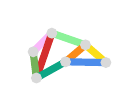
\begin{tikzpicture}[x=0.09pt,y=0.09pt]
\definecolor{gA}{rgb}{0.98,0.72,0.98}
\definecolor{gB}{rgb}{0.83,0.18,0.18}
\definecolor{gC}{rgb}{0.55,0.95,0.60}
\definecolor{gD}{rgb}{0.45,0.70,0.35}
\definecolor{gE}{rgb}{0.05,0.65,0.52}
\definecolor{gF}{rgb}{0.98,0.55,0.10}
\definecolor{gG}{rgb}{0.98,0.87,0.10}
\definecolor{gH}{rgb}{0.30,0.55,0.92}
\draw[gA,line width=2.6pt] (25,128) -- (100,203);
\draw[gB,line width=2.6pt] (100,203) -- (38,23);
\draw[gC,line width=2.6pt] (100,203) -- (235,156);
\draw[gD,line width=2.6pt] (25,128) -- (38,23);
\draw[gE,line width=2.6pt] (38,23) -- (155,88);
\draw[gF,line width=2.6pt] (155,88) -- (235,156);
\draw[gG,line width=2.6pt] (235,156) -- (317,85);
\draw[gH,line width=2.6pt] (155,88) -- (317,85);
\fill[black!15] (100,203) circle (22);
\fill[black!15] (25,128) circle (22);
\fill[black!15] (235,156) circle (22);
\fill[black!15] (155,88) circle (22);
\fill[black!15] (317,85) circle (22);
\fill[black!15] (38,23) circle (22);
\end{tikzpicture}%%
}};
\node[capt, anchor=north, color=ink] at (3.39, {\zt-0.52}) {\texttt{pdbe-arpeggio}};

% ---------- barramento -> tres alvos ----------
\draw[sflow] (4.72, \zt) -- (5.13, \zt);
\draw[sbus]  (5.15, \zc) -- (5.15, \zd);
\foreach \zz in {\zc, \zt, \zd}{\draw[sflow] (5.15, \zz) -- (5.91, \zz);}

\begin{scope}[shift={(5.95, {\zc+\hw/2})}]
  \lmap{\hs}{6}{contextfill}{\ctc}
  \node[capt, anchor=north] at ({\hw/2}, {-\hw-0.06}) {contact};
\end{scope}
\begin{scope}[shift={(5.95, {\zt+\hw/2})}]
  \foreach \kk/\oo in {7/0.28, 6/0.24, 5/0.20, 4/0.16, 3/0.12, 2/0.08, 1/0.04}{
    \fill[contextfill, draw=context, line width=0.4pt]
      ({\oo},{-\oo}) rectangle ({\oo+\hw},{-\oo-\hw});}
  \begin{scope}\lmap{\hs}{6}{muted}{\ctc}\end{scope}
  \node[capt, anchor=north] at ({\hw/2+0.14}, {-\hw-0.34}) {\textbf{8 types}};
\end{scope}
\begin{scope}[shift={(5.95, {\zd+\hw/2})}]
  \lmap{\hs}{6}{contextfill}{\ctc}
  \node[capt, anchor=north] at ({\hw/2}, {-\hw-0.06}) {distance};
\end{scope}

% ---------- tres alvos -> loss (barramento convergente) ----------
\foreach \zz in {\zc, \zd}{\draw[sbus] (6.76, \zz) -- (7.60, \zz);}
\draw[sbus] (7.04, \zt) -- (7.60, \zt);
\draw[sbus] (7.60, \zc) -- (7.60, \zd);
\draw[sflow] (7.60, \zt) -- (9.72, \zt);

\node[capt, anchor=west, align=left, inner sep=1.2pt] at (9.86, \zt)
     {loss\\\tiny BCE $+$ ASL $+$ 0.1$\cdot$MSE};

% ---------- unica travessia: continua a espinha do registro superior ----------
\draw[{Straight Barb[length=2.6pt,width=3.2pt]}-, draw=context, line width=1.0pt,
      dash pattern=on 3pt off 2pt]
  (\bus, \yd) -- (\bus, -3.52);
\node[capt, anchor=west, align=left] at ({\bus+0.14}, -2.62) {gradient};

\end{tikzpicture}}
  \caption{Above the barrier, the input path; below it, the supervision that
  \texttt{pdbe-arpeggio} derives from the 3D structure. At inference the lower half is
  absent. The three icons come from the same
  test chain (6AVD\_A, 40 residues, 8 cysteines): the cysteines highlighted in the
  sequence are the nodes of the four disulfide bridges that reappear in the
  cartoon and as predicted \texttt{covalent} edges. The RIN on the right is model
  output ($p>0.5$), not annotator label.}
  \label{fig:pipeline}
\end{figure}

\section{Materials and Methods}
\label{sec:methods}

\subsection{Data and anti-leakage protocol}
\label{sec:dataset}

X-ray structures were retrieved from the Protein Data Bank
(PDB)~\cite{berman2000pdb} using its search interface and filtered to resolution
$\leq 2.5$\,\AA, one protein entity, 30--350 residues and one deposited model. Intra-chain scope is enforced at labelling time: one chain per entry, and an
interaction is kept only when both atoms share the same \texttt{auth\_asym\_id} and
Arpeggio reports \texttt{INTRA\_SELECTION}. The most consequential decision is
deduplication. One representative is retained from each 30\%-identity cluster, so no
retained chains share a cluster; the representatives are split into 3,962 training, 495
validation and 496 test chains, of which 494 are evaluated after two label-length
mismatches are removed. Without it, near-identical
homologues would fall on both sides of the split and inflate every metric.

Labels come from \texttt{pdbe-arpeggio}~\cite{jubb2017arpeggio} over mmCIF files: atoms
map to residues and type labels are combined by logical OR for each pair. Water is
discarded, as are all pairs with $|i-j|<3$. Of the 11 raw types, eight are retained
($T=8$): \texttt{xbond} and \texttt{metal} have zero examples, whereas
\texttt{proximal} occurs on 99.995\% of edges and is effectively redundant with contact
existence. The difficulty follows from two scales that multiply. Only 4.01\% of the 40,088,397
valid training pairs are edges, and within them the classes span a
392-fold range, from \texttt{polar} at 638,361 positives to \texttt{covalent} at 1,628.
Classes are not mutually exclusive: the class counts sum to 105.19\% of the edge count,
or 1.05 types per edge. Training-set prevalences appear in
Table~\ref{tab:perclass}.

\subsection{Sequence-only inputs and architecture}
\label{sec:model}


Figure~\ref{fig:pipeline} separates the two paths that meet only at the loss. The
sequence-derived inputs are the ESM-2 embedding, its attention-derived contact map, the
amino-acid (AA) identities of the residue pair and $\log(1+|i-j|)$; Arpeggio-derived
annotations serve only as targets, entering solely through the supervised loss.
Chains are encoded with ESM-2 650M~\cite{lin2023esm2} (layer 33, $d=1280$), frozen,
since the question is how much an off-the-shelf representation already encodes. The
\texttt{PairConv2D} head projects 1280 to 32 dimensions, forms an $L{\times}L$ map by
outer product and applies a dilated 2D ResNet, with heads for contact, for the $T=8$
types and for distance. All the inputs but the embedding enter as extra channels of
that map, \emph{outside} the projection. The head has 939,026 trainable parameters, under 0.15\% of the encoder.

Training uses $64{\times}64$ crops biased towards positives and rare classes, with
per-class weights capped at 8 and the Asymmetric Loss
(ASL)~\cite{ridnik2021asl}, which decouples the positive and negative focusing
exponents and so suppresses abundant negatives without suppressing rare positives. The
loss combines contact binary cross-entropy, type ASL and 0.1 times the distance mean
squared error.

\subsection{Evaluation protocol and baselines}
\label{sec:eval}

Evaluation includes every valid test pair, without negative sampling: 5,176,314 pairs
with 206,700 contacts (3.99\%). The metric is macro AUPRC, the unweighted mean over the
eight classes, so rare and frequent classes weigh equally. For AUPRC a random classifier
scores the class prevalence, not 0.5, giving macro chance 0.005; 95\% confidence
intervals (CIs) come from bootstrapping \emph{chains}, not pairs ($B=1000$). One caveat
governs the reading: the ablation ladder was scored under this same evaluation, so the
final value is \emph{selected on the test set}, with validation used only to monitor the
train--validation gap. With no direct competitor, two baselines test the strongest
alternative explanations. The contact oracle scores every type with the \emph{true}
contact label and cannot rank types among contacts, because its per-class AUPRC equals
test-set prevalence divided by contact density, a \emph{constant} $25.0\times$ lift in
all eight classes; it is a rescaled chance floor, and a ceiling only for binary-scoring
methods. The propensity baseline estimates
$P(t \mid aa_i, aa_j, \mathrm{range}(|i-j|))$ from training counts. The contact-head
score (\textsc{p-contact}) is an ablation, not a baseline.

\section{Results}
\label{sec:results}

\subsection{Comparison with the contact map: information content and oracle}
\label{sec:thesis}

The information-theoretic result uses only the labels. Of the 206,700 test contact edges,
36.9\% carry none of the eight types, and each edge carries 1.06 types on average.
Summing the eight binary entropies conditioned on contact gives 3.209 bits per edge;
because label correlation is ignored, that sum is only an upper bound. The joint entropy
is bounded below by the largest marginal, \texttt{polar} at 0.97 bit. A \emph{perfect}
contact map therefore leaves between 0.97 and 3.209 bits per edge unresolved, and both
bounds are far from the zero that would make the RIN a relabelling of proximity.

The sequence-only model reaches macro AUPRC 0.520 (95\% CI $[0.506, 0.535]$) against
0.132 for the oracle, a factor of 3.9. However, the macro average hides the class-wise
pattern (Table~\ref{tab:perclass}). Except for \texttt{hbond}, the model-to-oracle
ratio grows with class rarity: $2.0\times$ in \texttt{polar},
$28\times$ in \texttt{ionic}, $51\times$ in \texttt{aromatic} and $800\times$ in
\texttt{covalent}. This model-to-oracle gap is not an artefact
of the binary score: the continuous \textsc{p-contact} performs better (0.174) but
remains $3.0\times$ below. Against the \emph{strongest} alternative in each class the
model outperforms all eight, by margins from $1.2\times$ to $8.7\times$.

\begin{table}[tb]
\centering
\caption{Per-class AUPRC on the 494 test chains. \emph{Train prev.} is the training-set
prevalence, given for the imbalance scale; the chance floor here is the test prevalence
(Section~\ref{sec:eval}). \emph{Oracle}, \textsc{p-contact} and \emph{Prop.} are the
perfect contact map, the contact head and the propensity table.
\colorbox{accentfill}{Blue} is SPIN-Seq; \colorbox{contextfill}{grey} is the strongest
alternative in the row, the denominator of \emph{Gain}.}
\label{tab:perclass}
\scriptsize
\renewcommand{\arraystretch}{1.0}
\setlength{\tabcolsep}{4.4pt}
\begin{tabular}{lrrrr>{\columncolor{accentfill}}l>{\columncolor{accentfill}}r}
\toprule
\rowcolor{cabec}
Class & Train prev. & Oracle & \textsc{p-contact} & Prop. & SPIN-Seq \tiny[95\% CI] & Gain \\
\midrule
\texttt{covalent}    & 0.00004 & 0.001 & 0.001 & \cellcolor{contextfill}0.092 & 0.801 \tiny[0.727, 0.868] & 8.7$\times$ \\
\texttt{aromatic}    & 0.00041 & 0.009 & 0.006 & \cellcolor{contextfill}0.077 & 0.461 \tiny[0.432, 0.490] & 6.0$\times$ \\
\texttt{hbond}       & 0.00047 & 0.010 & \cellcolor{contextfill}0.014 & \cellcolor{contextfill}0.014 & 0.069 \tiny[0.049, 0.097] & 4.9$\times$ \\
\texttt{ionic}       & 0.00056 & 0.014 & 0.011 & \cellcolor{contextfill}0.083 & 0.394 \tiny[0.370, 0.416] & 4.7$\times$ \\
\texttt{carbonyl}    & 0.00145 & 0.035 & \cellcolor{contextfill}0.057 & 0.009 & 0.359 \tiny[0.339, 0.378] & 6.3$\times$ \\
\texttt{vdw}         & 0.01166 & 0.292 & \cellcolor{contextfill}0.425 & 0.210 & 0.681 \tiny[0.667, 0.695] & 1.6$\times$ \\
\texttt{hydrophobic} & 0.01172 & \cellcolor{contextfill}0.295 & 0.212 & 0.098 & 0.599 \tiny[0.583, 0.615] & 2.0$\times$ \\
\texttt{polar}       & 0.01592 & 0.401 & \cellcolor{contextfill}0.669 & 0.299 & 0.796 \tiny[0.782, 0.809] & 1.2$\times$ \\
\midrule
\textbf{macro} & \textbf{0.00528} & \textbf{0.132} & \cellcolor{contextfill}\textbf{0.174} & \textbf{0.110} & \textbf{0.520} \tiny[0.506, 0.535] & \textbf{3.0}$\times$ \\
\bottomrule
\end{tabular}
\end{table}


\subsection{Comparison with amino-acid propensity}
\label{sec:notcomposition}

A second alternative is compositional: since \texttt{ionic} bonds pair an acidic residue
(D/E) with a basic one (K/R/H), and \texttt{covalent} bonds join two cysteines, a lookup
table might reproduce the result without context. The model outperforms the propensity baseline by
$+0.410$ (0.520 against 0.110, 95\% CI $[0.395, 0.424]$); all nine comparisons are
significant at the resampling floor $p=1/B=0.001$. That baseline is strong exactly where chemistry predicts,
beating the oracle on \texttt{ionic} (0.083), \texttt{aromatic} (0.077) and
\texttt{covalent} (0.092): the explanations are complementary and the model beats both. Treating the chemical rules as filters clarifies why. Cys--Cys pairs cover 97.7\% of the
\texttt{covalent} edges but only 7.7\% of candidate Cys--Cys pairs bond; the D/E--K/R/H rule covers 99.5\%
of the \texttt{ionic} edges, yet only 1.5\% of its 189,006 admissible pairs are salt
bridges. Composition says fairly precisely \emph{where to look} and little about \emph{which
pair to select}. Combining the two was not evaluated, and may account for part of the gain.

\subsection{Ablation, model capacity and learning curve}
\label{sec:ablation}

\begin{table}[tb]
\centering
\caption{Ordered ablation ladder on 494 test chains. \emph{Contact} and \emph{Macro}
are AUPRC; the ladder is descriptive, since the final recipe was selected on this same
evaluation. \colorbox{accentfill}{Blue} is the headline metric, \colorbox{queda}{red}
the only decreases, \colorbox{alta}{green} their recovery once the explicit AA-pair
feature is added.}
\label{tab:ablation}
\scriptsize
\renewcommand{\arraystretch}{1.0}
\setlength{\tabcolsep}{5pt}
\begin{tabular}{llc>{\columncolor{accentfill}}crr}
\toprule
\rowcolor{cabec}
Step & Change & Contact & Macro & ionic & aromatic \\
\midrule
0 & Pair MLP                            & 0.718 & 0.429 & 0.363 & 0.363 \\
1 & $L{\times}L$ map + ResNet        & 0.814 & 0.440 & \cellcolor{queda}0.248\,$\downarrow$ & \cellcolor{queda}0.120\,$\downarrow$ \\
2 & Class-weight cap $3\to8$          & 0.815 & 0.460 & 0.270 & 0.204 \\
3 & ASL instead of focal loss    & 0.815 & 0.478 & 0.298 & 0.289 \\
4 & \textbf{AA pair feature}            & \textbf{0.815} & \textbf{0.520} \tiny$[0.506,0.535]$ & \cellcolor{alta}\textbf{0.394}\,$\uparrow$ & \cellcolor{alta}\textbf{0.461}\,$\uparrow$ \\
\bottomrule
\end{tabular}
\end{table}

A pairwise multilayer perceptron (MLP) on the same frozen embedding already reaches
macro 0.429, itself $3.25\times$ the perfect-contact oracle, and the remaining steps add
0.091: the thesis does not rest on the head architecture. Within the ladder the two
tasks behave as largely separable (Table~\ref{tab:ablation}). Step~1 accounts for
almost the entire contact gain and almost none of the chemistry; the later steps leave
contact flat at 0.815 while the macro climbs from 0.440 to 0.520. The 1280-to-32
projection of step~1 omits the explicit AA-pair feature, and \texttt{ionic} and
\texttt{aromatic} \emph{fell} at the step that produced the largest contact gain; these
were the ladder's only decreases. Adding that feature \emph{outside} the projection
(step~4) raised the macro from 0.478 to 0.520, concentrated in the classes the chemical
hypothesis predicts (\texttt{aromatic} $+0.172$, \texttt{ionic} $+0.096$, \texttt{polar}
within seed noise) rather than spread uniformly, as generic capacity would give.

Widening the projection to 128 reduced contact/macro AUPRC to 0.801/0.500 with no class
improving, and the train--validation gap rose from 0.026 to 0.058. The learning curve
over nested training subsets slows early but shows no resolved saturation: the slope with
respect to $\ln(n)$ falls from 0.076 to 0.037, while the third segment, 0.038, is
indistinguishable from the second within seed noise, with the gains from added data
concentrated in the rare classes.

The selection query leaves 5,926 unused clusters; including them would yield $2.2\times$
as many clusters as the 4,953 used here, without relaxing the filters. A log-linear fit over four points
($R^2=0.967$) extrapolates to $\approx0.57$ and the last observed segment to
$\approx0.55$, but neither the functional form nor saturation is resolved. Over three seeds
the recipe yields macro $0.518 \pm 0.003$ (standard deviation across seeds, not the
bootstrap CI); the 0.520 quoted throughout is the reference seed, and differences below
$\approx0.01$ are treated as unresolved.

\section{Discussion}
\label{sec:discussion}

The value 0.520 must be read against a macro chance of 0.005 and a \emph{perfect}
contact map at 0.132. The \texttt{hbond} class is the main low-performing one, and its
result (0.069) is treated here as an open challenge; excluding it, the mean over the
other seven is 0.584. Re-deriving labels with Arpeggio's hydrogen-minimisation protocol
over 119 structures changes \texttt{hbond} only modestly (Jaccard 0.967, against exactly
1.000 for the other eight non-empty Arpeggio types, \texttt{proximal} included), so that
perturbation does not explain the low AUPRC. The final data increase gave no resolved
gain either: although \texttt{hbond} has $11.6\times$ more examples than
\texttt{covalent}, its AUPRC is about one eleventh as large. Under this representation,
architecture and annotation convention the class remains poorly resolved, and the
evidence does not distinguish a limit of sequence information from limitations of the
frozen readout or of Arpeggio's convention.

Five limitations bound the results. The analysis covers 30--350-residue single chains
resolved by X-ray at $\leq 2.5$\,\AA, and the labels come from one annotation tool, not
from direct measurement. The frozen encoder was pretrained on UniRef, which likely
contains the test sequences, and its contact readout was fitted on PDB structures, so
the cluster-disjoint split removes leakage into the trained head, not into the
representation. The eight-type vocabulary is not exhaustive: 36.9\% of test contacts
receive none. Finally, the fold-and-profile route was not run, so that argument remains
untested on the same chains.

\section{Conclusion and future work}
\label{sec:conclusion}

The results show that the typed RIN is predictable from sequence alone and is a target
distinct from the contact map. On the reference seed and over 5,176,314 pairs, SPIN-Seq
reaches macro AUPRC 0.520 against 0.132 for a perfect contact map, with the gap over the
oracle generally widening as classes become rarer. Locating a contact and typing it behave as separable, and the largest chemical
gain occurs when the explicit AA-pair feature is added outside the projection.

Since the tested width increase produced no gain and the learning-curve slope has not resolvably fallen
to zero, the priority is to expand training with the 5,926 unused clusters while reserving a
fresh cluster-disjoint test split, since the current test chains already informed recipe
selection. Future work will also compare SPIN-Seq with the fold-and-profile route. Code, per-split chain
lists and raw evaluation outputs are available at
\url{https://github.com/labitec-cloud/SPIN-Seq}.

{\footnotesize
\bibliographystyle{sbc}
\bibliography{sbc-template}}

\end{document}
